In this section we provide a complete axiomatization of
multi-agent \textsc{EviL}.  In addition to axiomatics, we shall also
look at subsystems and supersystems of \textsc{EviL}, and provide
complexity bounds on \textsc{EviL} decision procedures. 

We have organized this section in the following manner:
\begin{description}
 \item[\S\ref{evil-axioms}] We first present a sound axiom
   system for \textsc{EviL}.

 \item[\S\ref{abstraction}] Next, we give a definition of the
   class of \emph{partly \textsc{EviL}} Kripke models.  

   We then reveal that \textsc{EviL} is sound and strongly complete
   for the class of partly \textsc{EviL} models. 
   Completeness rests on the observation that the
   axioms of \textsc{EviL} are all in the \emph{Sahlqvist fragment},
   or have obvious meanings in terms of the traditional canonical
   model construction for Modal Logic.
   This abstract completeness for \textsc{EviL} can be understood as
   an elementary application of van Benthem's 
   \emph{correspondence theory} for modal logic.

\item[\S\ref{completely-evil}]  In this section we recall the definition of an
  \emph{\textsc{EviL} Kripke Model}, as we gave in Definition
  \ref{evil-kripke-structures} from \S\ref{kripke}, and show that
  every \emph{partly \textsc{EviL}} Kripke model may be
  ``completed'' by constructing a bisimilar \emph{\textsc{EviL}} 
   model.

   This has, as a consequence, that \textsc{EviL} is complete for
   \textsc{EviL} Kripke Models.

\item[\S\ref{taking-stock}]  In this section, we discuss why the abstract
  completeness proof developed in the previous sections, while
  important, is not adequate in light of the developments in
  \S\ref{basic-evil} and the intuitions we saw in that section.  We
  shall sketch what further needs to be shown to give the desired
  completeness theorem for \textsc{EviL}.

\item[\S\ref{small-model}]  In this section we show that
  \textsc{EviL} has a small model property for \emph{partly
    \textsc{EviL}} Kripke models. This is accomplished by constructing
     a Kripke model consisting of finite maximally
     consistent sets in the manner of the Fischer-Ladner closure style
     completeness proof of PDL 
     \cite[chapter 4, pgs. 241--248]{blackburn_modal_2001}.

% \item[\S\ref{decidability}] 
%    From our construction in the previous section, we obtain a decidability
%    result for \textsc{EviL}, and provide upper and lower bounds on the
%    complexity of the \textsc{EviL} decision problem.

  \item[\S\ref{islands}] In this section, we introduce the concept of an
    \emph{island}, which are special equivalence classes for
    \textsc{EviL} models.  We shall prove several properties, which take the
    form of irreducibilities. 

\item[\S\ref{translation}]Following the proof of Proposition
  \ref{translation-sketch} in \S\ref{sketch}, we shall show that every
  finite \textsc{EviL} Kripke structure is \emph{(almost)-homomorphic} to another,
  \textsc{EviL} model we shall call $\ipent$, provided that we have an
  infinite number of letters in $\Phi$.  
  We shall show that there is a map $\kl$ of worlds in $\mathbb{M}$ to
  worlds in $\ipent$ that preserves formulae in a language
  $\mathcal{L}(\Psi,\mathcal{A})$ where 
$\Psi \subseteq_\omega \Phi$.

  The construction of $\ipent$ shall make use of the island structures introduced
  in the previous section, and here we will also introduce the concept of
  \emph{names} and \emph{surnames}.

We have, as a consequence of the above, we shall be able to show that
$\textsc{EviL}$ is weakly complete for $\textsc{EviL}$ models.

  % \item[\S\ref{skarmy-of-darkness}]  In this section, we employ our
  %   previous results to remark that \textsc{EviL} is weakly complete for
  %   \textsc{EviL} models.

\item[\S\ref{taking-stockII}]  In this section, we once again pause to
  take stock of the results we have established in previous sections.
  We discuss how our results give rise to complexity observations for
  \textsc{EviL}, and discuss the relationship between the abstract
  completeness we have previously established and our concrete 
  completeness.

  \item[\S\ref{subsystems}] We next introduce two
    subsystems of \textsc{EviL}, corresponding to the $\BP$ and $\BM$
    only fragments. We briefly go over the completeness theorems and
    finite model property for these systems.  In each case, a special
    bisimulation theorem is in order to achieve completeness.

  \item[\S\ref{supersystems}] We provide an extension to
    \textsc{EviL} and its subsystems, introducing the universal
    modality $U$. We sketch completeness and the finite model
    property, and mention how translation may be extended to this
    system.

 \item[\S\ref{lattice}]  In this section we give a lattice of
   \textsc{EviL} systems, and discuss the known complexity bounds of
   various levels of this lattice.
\end{description}

%\subsubsection{Failure of Compactness}
%\label{non-compactness}
%In this section I shall demonstrate that \textsc{EviL} is not compact by giving an example of an infinite set of formulae for which every finite subset is satisfiable while the entirety is not.

\begin{lemma}
Let $\tau : \Phi \to \mathcal{L}$ be defined as follows:
\begin{center}
\begin{minipage}{3in}
\begin{tabbing}
	$\tau(p) := $ \=$p \wedge \Pos\top \wedge$ \\
	\> $\Nec$ \= $(\neg p \wedge \Pos\top \wedge$\\
	\> \> $\Nec$ \= $(p \wedge \Pos p))$
\end{tabbing}
\end{minipage}
\end{center}
Every finite subset of $\tau[\Phi]$ is satisfiable, but not the entirety, which is infinite. 
\end{lemma}
\begin{proof}
That $\tau[\Phi]$ is infinite is immediate, as $\Phi$ was stipulated to be infinite. 

So let $S\subseteq \tau[\Phi]$ by finite.  We shall find a model that
satisfies $S$.  First observe that there is a
 finite $\Psi\subset
\Phi$ such that $S = \tau[\Psi]$.  Let $\{q,r,s\} \subseteq \Phi \; \bs
\; \Psi$ be
 three distinct letters - this can be done, since $\Phi \;
\bs \; \Psi$ is infinite.
  Let $\mathfrak{M} = \{\pr{a}{\{q\}},
\pr{b}{\{r\}}, \pr{c}{\{s\}} \}$, where 
\begin{align*}
a & := \Psi \cup \{s\} \\
b & := \{q \} \\
c & := \Psi \cup \{r\}
\end{align*}
 Using the same visualizations I introduced in \S\ref{contradictions},
 $\mathfrak{M}$ can  be visualized\footnote{While this situation
   presents itself like a Kripke model, I am not employing Kripke
   semantics.  The means in which one world accesses another is not by
   an accessibility relation, but rather through the sets of beliefs,
   which in this case are the sets ${q},{r},$ and ${s}$.} in Fig. \ref{fig:mod4}.  It is straightforward to 
check that $\mathfrak{M},( a,\{q\}) \VDash \tau(p)$ for all $p \in \Psi$.

	\begin{figure}[htbp] %  figure placement: here, top, bottom, or page
   \centering
	\begin{tikzpicture}[->,
         shorten >=3pt, shorten <= 3pt, 
         auto,node distance=4cm, semithick]
  \tikzstyle{state}=[draw=black, shape=rectangle]
  \tikzstyle{empt} = [draw=none,fill=none]
\begin{scope}
\node[state] (aA1) at (45:2.5) [] {$\pr{a}{\{q\}}$};
\node[empt] (aA2) at (165:2.5) {$\pr{b}{\{r\}}$};
\node[empt] (aA3) at (285:2.5) {$\pr{c}{\{s\}}$};
\path
(aA1) edge [->,bend right] node {} (aA2)
(aA2) edge [->,bend right] node {} (aA3)
(aA3) edge [->,bend right] node {} (aA1);
\end{scope}
\end{tikzpicture}
\caption{$\mathfrak{M},\pr{a}{\{q\}}\VDash \tau[\Psi]$}
   \label{fig:mod4}
\end{figure}
On the other hand, suppose there was some model $\mathfrak{N}$ such that $\mathfrak{N}, ( a, A) \VDash \tau(p)$ for all $p \in \Psi$.
This implies that $\mathfrak{N}, ( a, A) \VDash p$ for each $p \in
\Phi$.  Moreover, let $( b, B)\in\mathfrak{N}$ be such that $b \models A$ 
(one exists since by hypothesis $\mathfrak{N}, ( a, A)
\VDash \Pos p$).  By the semantics of $\tau(p)$, it is evident that
$\mathfrak{N}, ( b, B) \VDash \neg p$ and that there's a $( c, C)\in\mathfrak{N}$
such that $c \models B$ and $\mathfrak{N},( c,C )
\VDash p \wedge \Pos p$.  But then from this it must be that $a$ and
$c$ both contain exactly the same sentence letters, so $a = b$ which means that
$a \models B$ as well, since $B \subseteq
\mathcal{L}_0$ (as per the grammar restriction).  However it cannot be that
$\mathfrak{N},( a,A ) \VDash \Pos p$ since $\mathfrak{N},( a,A )
\VDash \Nec \neg p$, which follows from the assumption that $\mathfrak{N},( a,A )
\VDash \tau(p)$. 
Thus it is impossible that $\mathfrak{N},( a, A) \VDash \tau[\Phi]$. $\lightning$
\end{proof}

The above argument illustrates that while \textsc{EviL} semantics
present themselves as similar to the traditional Kripke Semantics for modal
logic, they aren't the same.  If for some reason two world-pairs
$(a,A)$ and $(b,B)$ make true the same sentence letters, then $a=b$,
and then for any $C \subseteq \mathcal{L}_0$, we have that $a \models
C$ if and only if $b \models C$. This is crucial - even though
\textsc{EviL} is modal, it has no accessibility relations; the role of
accessibility relations is instead picked up by sets of beliefs $C$. 
Since my initial design considerations for \textsc{EviL} demanded a
grammar restriction, to ensure the semantics were well-defined,
an unusual failure of compactness manifests itself.

My failure of compactness, while a fairly basic result in the model
theory of \textsc{EviL}, has far reaching consequences for the model
theory of \textsc{EviL}.  As a consequence, there is
no hope of achieving completeness using infinitary Lindenbaum
constructions that are typically employed in modal logic, such as is
done in \citep[][chapter 4]{blackburn_modal_2001}, for instance.
Hence the completeness theorem for \textsc{EviL} presented in \S\ref{army-of-darkness}
will necessarily have to be finite in nature.
%%% Local Variables: 
%%% mode: latex
%%% TeX-master: "evil_philosophy"
%%% End: 


\subsubsection{Axioms of \textsc{EviL}}\label{evil-axioms}
In this section, we shall present the axiom system which represents
the validities of \textsc{EviL} semantics as provided in . 

Table \ref{table:axioms}, provides a Hilbert-style axiom system for \textsc{EviL}.  In addition to giving each axiom, we have also provided our own philosophical reading of what each axiom says.  One unusual feature of this logic is that it is not \emph{normal}, that is it is not closed under variable substitution.

\begin{table}
\newcounter{rownum}
\setcounter{rownum}{0}
\newcounter{rownum2}
\setcounter{rownum2}{0}
\begin{tabularx}{\linewidth}{|cl>{\it}X|}
\hline
(\refstepcounter{rownum}\arabic{rownum}) & $\vdash \phi \to \psi \to \phi$ & \multirow{3}{*}{Axioms for basic propositional logic} \\
(\arabic{rownum}) & $\vdash (\phi \to \psi \to \chi) \to (\phi \to \psi) \to \phi \to \chi$ &  \\
(\refstepcounter{rownum}\arabic{rownum}) & $\vdash (\neg \phi \to \neg \psi) \to \psi \to \phi$ &  \\[6pt]
(\refstepcounter{rownum}\arabic{rownum}\label{reflAx})
 & $\vdash \BBI_X \phi \to \phi$ & If $\phi$ holds under any further evidence $X$ considers, then $\phi$ holds simpliciter, since considering no additional evidence is trivially considering further evidence \\[6pt]
(\refstepcounter{rownum}\arabic{rownum})\label{transAx} & $\vdash \BBI_X \phi \to \BBI_X \BBI_X \phi$ & If $\phi$ holds under any further evidence $X$ considers, then $\phi$ holds whenever $X$ considers even further evidence beyond that \\[6pt]
(\refstepcounter{rownum}\arabic{rownum})\label{letterAx1} & $\vdash p \to \BB_X p$ & \multirow{2}{8.5cm}{Changing one's mind does not bear on matters of fact}\\
(\refstepcounter{rownum}\arabic{rownum})\label{letterAx2} & $\vdash p \to \BBI_X p$ & \\[6pt]
(\refstepcounter{rownum}\arabic{rownum})\label{downConceive} & $\vdash \Pos_X \phi \to \BB_X \Pos_X \phi$ & The more evidence $X$ discards, the freer her imagination can run \\[6pt]
(\refstepcounter{rownum}\arabic{rownum})\label{islandDown} & $\vdash \Nec_X \phi \to \Nec_X \BB_Y \phi$ &  \multirow{2}{8.5cm}{If $X$ believes a proposition, she believes it regardless of what anyone else thinks} \\
(\refstepcounter{rownum}\arabic{rownum})\label{islandUp} & $\vdash \Nec_X \phi \to \Nec_X \BBI_Y \phi$ & \\[6pt]
(\refstepcounter{rownum}\arabic{rownum})\label{soundness} & $\vdash \PP_X \to \Nec_X \phi \to \phi$ & If $X$'s premises are sound, then her logical conclusion are correct \\[6pt]
(\refstepcounter{rownum}\arabic{rownum})\label{downsound} & $\vdash \PP_X \to \BB_X \PP_X $ & If $X$'s premises are sound then any subset will be sound as well \\[6pt]
(\refstepcounter{rownum}\arabic{rownum})\label{reverseAx1} & $\vdash \phi \to \BB_X \DDI_X \phi$ &
\multirow{2}{8.5cm}{Embracing evidence is the inverse of discarding evidence} 
\\
(\refstepcounter{rownum}\arabic{rownum})\label{reverseAx2} & $\vdash \phi \to \BBI_X \DD_X \phi$ & \\[6pt]
(\refstepcounter{rownum}\arabic{rownum}) & $\vdash \Nec_X (\phi \to \psi) \to \Nec_X \phi \to \Nec_X \psi$ &
\multirow{3}{8.5cm}{Variations on axiom $K$}
\\
(\refstepcounter{rownum}\arabic{rownum}) & $\vdash \BB_X (\phi \to \psi) \to \BB_X \phi \to \BB_X \psi$ & \\
(\refstepcounter{rownum}\arabic{rownum}) & $\vdash \BBI_X (\phi \to \psi) \to \BBI_X \phi \to \BBI_X \psi$ & \\[6pt]
(\refstepcounter{rownum2}\Roman{rownum2}) & 
 $\AxiomC{$\vdash \phi \to \psi$}
\AxiomC{$\vdash \phi$}
\BinaryInfC{$\vdash \psi$}
\DisplayProof$ & Modus Ponens\\[10pt]
(\refstepcounter{rownum2}\Roman{rownum2}) & 
 $\AxiomC{$\vdash \phi$}
\UnaryInfC{$\vdash \Box_X \phi$}
\DisplayProof$ & \multirow{3}{8.5cm}{Variations on necessitation}\\
(\refstepcounter{rownum2}\Roman{rownum2}) \label{BMnec}& 
 $\AxiomC{$\vdash \phi$}
\UnaryInfC{$\vdash \BB_X \phi$}
\DisplayProof$ &  \\
(\refstepcounter{rownum2}\Roman{rownum2}) &
 $\AxiomC{$\vdash \phi$}
\UnaryInfC{$\vdash \BBI_X \phi$}
\DisplayProof$ & \\[10pt]
\hline
\end{tabularx}
\caption{A Hilbert style axiom system for \textsc{EviL}}
\label{table:axioms}
\end{table}


%%% Local Variables: 
%%% mode: latex
%%% TeX-master: "../evil_philosophy"
%%% End: 


This logic makes true a variety of relationships between the various
modalities, which are given in the following lemma:
\begin{lemma}\label{equivs}
We have the following provable equivalences:
\begin{eqnarray*} \vdash \Nec_X \phi \IFF \BB_X \Nec_X \phi & \hspace{1cm} \vdash \Nec_X \phi \IFF \Nec_X \BB_Y \phi \hspace{1cm}  & \vdash \Nec_X \phi \IFF \Nec_X \BBI_Y \phi \\
 \vdash \BB_X \phi \IFF \BB_X \BB_X \phi & \vdash \BBI_X \phi \IFF \BBI_X \BBI_X \phi & \vdash \PP_X \IFF \BB_X \PP_X\end{eqnarray*}
%&\vdash \PP_X \IFF \DDI_X \PP_X \\
%&\vdash \phi \IFF \psi \textup{ implies } \vdash \chi \IFF \chi[\phi/\psi]
%\end{eqnarray*}
%\ldots where $\chi[\phi/\psi]$ is the same as $\chi$ but every occurrence of $\phi$ as a subformula is replaced by $\psi$.
%$\hfill\dashv$
\end{lemma}

In addition to the main system presented above, it can be understood to contain two subsystems, corresponding to two fragments of the main grammar:
\begin{definition}
Define $\mathcal{L}^\boxminus (\Phi, \mathcal{A})$ as the fragment:
\[ \phi \ {::=} \  p \in \Phi \  | \  \phi
   \rightarrow \psi \  | \  \bot \  |
   \  \Box_X \phi \  | \  \boxminus_X \phi
%   \  | \  \boxplus_X \phi
 \  | \ 
   \circlearrowleft_X \]

And define $\mathcal{L}^\boxplus (\Phi, \mathcal{A})$ as the fragment:
%Define $\mathcal{L}^\boxminus (\Phi, \mathcal{A})$ as the fragment:
\[ \phi \ {::=} \  p \in \Phi \  | \  \phi
   \rightarrow \psi \  | \  \bot \  |
   \  \Box_X \phi 
%\  | \  \boxminus_X \phi
   \  | \  \boxplus_X \phi
 \  | \ 
   \circlearrowleft_X \]
\end{definition}

Table \ref{table:axiomsII} gives the axioms systems for these two fragments.  For now, we shall observe that \textsc{EviL} extends \textsc{EviL}$^\BM$ and \textsc{EviL}$^\BP$.  In \S\ref{conservative-extension} we shall make this precise. 
\begin{table}
\begin{minipage}[b]{0.5\linewidth}
\centering
%\newcounter{rownum}
\setcounter{rownum}{0}
%\newcounter{rownum2}
\setcounter{rownum2}{0}
\begin{tabular}{|ll|}
\hline
  (\addtocounter{rownum}{1}\arabic{rownum})&$ \vdash \phi \rightarrow \psi \rightarrow \phi$\\
  (\addtocounter{rownum}{1}\arabic{rownum})&$ \vdash (\phi \rightarrow \psi \rightarrow \chi) \rightarrow (\phi
  \rightarrow \psi) \rightarrow \phi \rightarrow \chi$\\
  (\addtocounter{rownum}{1}\arabic{rownum})&$ \vdash (\neg \phi \rightarrow \neg \psi) \rightarrow \psi \rightarrow
  \phi$\\
  (\addtocounter{rownum}{1}\arabic{rownum})&$ \vdash \boxminus_X \phi \rightarrow \phi$\\
  (\addtocounter{rownum}{1}\arabic{rownum})&$ \vdash \boxminus_X \phi \rightarrow \boxminus_X \boxminus_X \phi$\\
  (\addtocounter{rownum}{1}\arabic{rownum})&$ \vdash p \rightarrow \boxminus_X p$\\
  (\addtocounter{rownum}{1}\arabic{rownum})&$ \vdash \neg p \rightarrow \boxminus_X \neg p$\\
  (\addtocounter{rownum}{1}\arabic{rownum})&$ \vdash \diamondsuit_X \phi \rightarrow \boxminus_X \diamondsuit_X \phi$\\
  (\addtocounter{rownum}{1}\arabic{rownum})&$ \vdash \Box_X \phi \rightarrow \Box_X \boxminus_Y \phi$\\
  (\addtocounter{rownum}{1}\arabic{rownum})&$ \vdash \phi \rightarrow \boxminus_X (\circlearrowleft_X \rightarrow
  \diamondsuit_X \phi)$\\
  (\addtocounter{rownum}{1}\arabic{rownum})&$ \vdash \circlearrowleft_X \rightarrow \boxminus_X \circlearrowleft_X$\\
  (\addtocounter{rownum}{1}\arabic{rownum})&$ \vdash \Box_X (\phi \rightarrow \psi) \rightarrow \Box_X \phi \rightarrow
  \Box_X \psi$\\
  (\addtocounter{rownum}{1}\arabic{rownum})&$ \vdash \boxminus_X (\phi \rightarrow \psi) \rightarrow \boxminus_X \phi
  \rightarrow \boxminus_X \psi$\\
(\addtocounter{rownum2}{1}\Roman{rownum2}) & 
 $\AxiomC{$\vdash \phi \to \psi$}
\AxiomC{$\vdash \phi$}
\BinaryInfC{$\vdash \psi$}
\DisplayProof$ \\ %& Modus Ponens\\[10pt]
(\addtocounter{rownum2}{1}\Roman{rownum2}) & 
 $\AxiomC{$\vdash \phi$}
\UnaryInfC{$\vdash \Box_X \phi$}
\DisplayProof$ \\ %& \multirow{3}{8.5cm}{Variations on necessitation}\\
(\addtocounter{rownum2}{1}\Roman{rownum2}) & 
 $\AxiomC{$\vdash \phi$}
\UnaryInfC{$\vdash \BB_X \phi$}
\DisplayProof$   \\
% (\addtocounter{rownum2}{1}\Roman{rownum2}) &
%  $\AxiomC{$\vdash \phi$}
% \UnaryInfC{$\vdash \BBI_X \phi$}
% \DisplayProof$  \\% [10pt]
\hline
\end{tabular}
\end{minipage}
\hspace{0.5cm}
\begin{minipage}[b]{0.5\linewidth}
 \centering
%\newcounter{rownum}
\setcounter{rownum}{0}
%\newcounter{rownum2}
\setcounter{rownum2}{0}
\begin{tabular}{|ll|}
\hline
  (\addtocounter{rownum}{1}\arabic{rownum})&$ \vdash \phi \rightarrow \psi \rightarrow \phi$\\
  (\addtocounter{rownum}{1}\arabic{rownum})&$ \vdash (\phi \rightarrow \psi \rightarrow \chi) \rightarrow (\phi
  \rightarrow \psi) \rightarrow \phi \rightarrow \chi$\\
  (\addtocounter{rownum}{1}\arabic{rownum})&$ \vdash (\neg \phi \rightarrow \neg \psi) \rightarrow \psi \rightarrow
  \phi$\\
  (\addtocounter{rownum}{1}\arabic{rownum})&$ \vdash \boxplus_X \phi \rightarrow \phi$\\
  (\addtocounter{rownum}{1}\arabic{rownum})&$ \vdash \boxplus_X \phi \rightarrow \boxplus_X \boxplus_X \phi$\\
  (\addtocounter{rownum}{1}\arabic{rownum})&$ \vdash p \rightarrow \boxplus_X p$\\
  (\addtocounter{rownum}{1}\arabic{rownum})&$ \vdash \neg p \rightarrow \boxplus_X \neg p$\\
  (\addtocounter{rownum}{1}\arabic{rownum})&$ \vdash \Box_X \phi \rightarrow \boxplus_X \Box_X \phi$\\
  (\addtocounter{rownum}{1}\arabic{rownum})&$ \vdash \Box_X \phi \rightarrow \Box_X \boxplus_Y \phi$\\
  (\addtocounter{rownum}{1}\arabic{rownum})&$ \vdash \phi \rightarrow \boxplus_X (\circlearrowleft_X \rightarrow
  \diamondsuit_X \phi)$\\
  (\addtocounter{rownum}{1}\arabic{rownum})&$ \vdash \neg \circlearrowleft_X \rightarrow \boxplus_X \neg
  \circlearrowleft_X$\\
  (\addtocounter{rownum}{1}\arabic{rownum})&$ \vdash \Box_X (\phi \rightarrow \psi) \rightarrow \Box_X \phi \rightarrow
  \Box_X \psi$\\
  (\addtocounter{rownum}{1}\arabic{rownum})&$ \vdash \boxplus_X (\phi \rightarrow \psi) \rightarrow \boxplus_X \phi
  \rightarrow \boxplus_X \psi$\\
(\addtocounter{rownum2}{1}\Roman{rownum2}) & 
 $\AxiomC{$\vdash \phi \to \psi$}
\AxiomC{$\vdash \phi$}
\BinaryInfC{$\vdash \psi$}
\DisplayProof$ \\ %& Modus Ponens\\[10pt]
(\addtocounter{rownum2}{1}\Roman{rownum2}) & 
 $\AxiomC{$\vdash \phi$}
\UnaryInfC{$\vdash \Box_X \phi$}
\DisplayProof$ \\ %& \multirow{3}{8.5cm}{Variations on necessitation}\\
% (\addtocounter{rownum2}{1}\Roman{rownum2}) & 
%  $\AxiomC{$\vdash \phi$}
% \UnaryInfC{$\vdash \BB_X \phi$}
% \DisplayProof$   \\
(\addtocounter{rownum2}{1}\Roman{rownum2}) &
 $\AxiomC{$\vdash \phi$}
\UnaryInfC{$\vdash \BBI_X \phi$}
\DisplayProof$  \\% [10pt]
\hline
\end{tabular}
\end{minipage}
\caption{Axiom system \textsc{EviL}$^\BM$ and \textsc{EviL}$^\BP$ respectively}
\label{table:axiomsII}
\end{table}

%%% Local Variables: 
%%% mode: latex
%%% TeX-master: "evil_philosophy"
%%% End: 


\subsubsection{Partly \textsc{EviL} Kripke Structures \& Strong Completeness}\label{abstraction}\label{partly-evil-strong-soundness-and-completeness}
In this section, we define what it means for a model to be
\emph{partly \textsc{EviL}}.  We should note that partly \textsc{EviL}
models are exactly the same as \textsc{EviL} models as defined in Definition
  \ref{evil-kripke-structures} from \S\ref{kripke}, only property
  \ref{pVII} has been weakened to \ref{ppVII} and \ref{ppIX}.

\begin{definition}[Partly \textsc{EviL}]\label{partly-evil}
A Kripke structure $\mathbb{M}=\langle W, R, \sqsubseteq, \sqsupseteq, V, P \rangle$ is called \textbf{partly
  \textsc{EviL}} whenever it makes true the following properties, for
all agents $\{X,Y\} \subseteq \mathcal{A}$:
  \begin{enumerate}[label=\textup{(\emph{\Roman*})$'$}, topsep=0.0in, parsep=0.075in]
    \item\label{ppI} $\sqsubseteq_X$ is reflexive
    \item \label{pptrans} $\sqsubseteq_X$ is transitive 
    \item \label{ppantisym} $\sqsubseteq$ is a partial order
    \item \label{ppreverse} $w \sqsubseteq_X v$ if and only if $v
    \sqsupseteq_X w$
    \item \label{islandiff} If $w \sqsubseteq_X v$ then ($w \in V (p)$ if and only if $v
    \in V (p)$)
    \item \label{ppV}$(R_X \circ \sqsubseteq_X) \subseteq
    R_X \subseteq (R_X \circ \sqsupseteq_X)$
    \item \label{ppVI} $(\sqsubseteq_Y \circ R_X) = R_X =
    (\sqsupseteq_Y \circ R_X)$
    \item\label{ppVII} If $w \in P_X$ then $w
    R_X w$
    \item\label{ppIX} If $w \in P_X$ and $w \sqsupseteq_X v$ then $v
    \in P_X$
  \end{enumerate}
\end{definition}

Note that it is elementary that every \textsc{EviL} structure is
partly \textsc{EviL} as well.

These properties are exactly the properties enforced
by the axioms of \textsc{EviL} given in Table \ref{table:axioms} in
\S\ref{evil-axioms}. We can see this by observing the following
theorem:

\begin{definition}\label{pEviL-Vdash}
We shall write
\[ \Gamma \Vdash_{\textup{p\textsc{EviL}}} \phi \]
to mean that for all partly \textsc{EviL} Kripke structures
$\mathbb{M} = \langle W, R, \sqsubseteq, \sqsupseteq, V, P \rangle$,
for all worlds $w \in W$ if $\mathbb{M},w \Vdash \Gamma$ then $\mathbb{M} \Vdash \phi$.
\end{definition}

\begin{theorem}[Partly \textsc{EviL} Strong Soundness and
  Completeness]\label{partly-evil-completeness}

$$\Gamma \vdash_{\textsc{EviL}} \phi\textup{ if and only if }\Gamma
\Vdash_{\textup{p\textsc{EviL}}} \phi$$

\end{theorem}
\begin{proof}
The left to right direction, \emph{soundness}, is trivial (one should
use induction).  So we shall focus on the right to left direction; 
to do this we shall consider the contrapositive.  We shall make heavy
use of \emph{correspondence} theory, namely the \emph{Sahlqvist
  Correspondence Theorem} \cite[Theorem 4.42,
pg. 212]{blackburn_modal_2001}.  We note that the axioms
\eqref{reflAx}, \eqref{transAx}, \eqref{downConceive}, \eqref{islandDown},
\eqref{islandUp}, \eqref{soundness}, \eqref{downsound},
\eqref{reverseAx1} and
\eqref{reverseAx2} are all
\emph{Sahlqvist formulae}.  When we say that a particular fact corresponds to an
axiom, we mean that from the Sahlqvist correspondence theorem and
first order logic one may be employed to show the fact in question.

So assume $\Gamma \nvdash \phi$, 
we must show that $\Gamma \nVdash \phi$.  
To see this, we carry out the canonical model construction as
described in \cite[chapter 4,
pgs. 198--422]{blackburn_modal_2001}\footnote{It is important to note
  that the results obtained in \cite{blackburn_modal_2001} are technically for any \emph{normal} modal logic,
  but they may be generalized to non-normal logics such as the
  \textsc{EviL} logic under consideration.}.  Let $\mathcal{E}$ be the set of maximally
  consistent sets of formulae for \textsc{EviL}. Define the
  \emph{canonical model}
  $$\mathscr{E} := 
\langle \mathcal{E}, R, \sqsubseteq, \sqsupseteq, V, P \rangle$$
where, for all $\{w,v\} \subseteq \mathcal{E}$:
\begin{bul}
  \item $w R_X v$ if and only if $\{ \phi\ |\ \Nec_X \phi \in w\}
    \subseteq v$
  \item $w \sqsubseteq_X v$ if and only if $\{ \phi\ |\ \BP_X \phi \in w\}
    \subseteq v$
  \item $w \sqsupseteq_X v$ if and only if $\{ \phi\ |\ \BM_X \phi \in w\}
    \subseteq v$
  \item $V(p) := \{ w \ |\ p \in w\}$
  \item $P_X := \{ w \ |\ \PP_X \in w \}$
\end{bul}

We know from the \emph{Lindenbaum Lemma} that $\Gamma$ may be extended
to some maximally consistent $\gamma$ such that $\Gamma \subseteq
\gamma$, $\gamma \in \mathcal{E}$ and $\phi \nin
\gamma$ \cite[Lemma 4.17,
pg. 199]{blackburn_modal_2001}.  By the \emph{Truth Lemma} we may establish
$\mathscr{E}, \gamma \nVdash \phi$ and $\mathscr{E}, \gamma \Vdash \Gamma$ \cite[Lemma 4.21,
pgs. 201]{blackburn_modal_2001}.  So it suffices to establish
that $\mathscr{E}$ is partly \textsc{EviL}, by establishing that it
satisfies the properties given in Definition \ref{partly-evil}.

  \begin{description}
    \item[\ref{ppI}] ``$\sqsubseteq_X$ is reflexive''
      corresponds from axiom \eqref{reflAx}.
    \item[\ref{pptrans}] ``$\sqsubseteq_X$ is transitive''
      corresponds to axiom \eqref{transAx}.
    \item[\ref{ppreverse}] ``$\sqsubseteq_X$ is the
      reverse $\sqsupseteq_X$'' corresponds to axioms \eqref{reverseAx1} and
      \eqref{reverseAx2}.
    \item[\ref{islandiff}] Assume $w \sqsubseteq_X v$, we shall show
      that 
$$w \in V (p)\textup{ if and only if }v \in V (p)$$
     Now assume that $w \in V(p)$, then $\mathscr{E}, w \Vdash p$.
      By axiom \eqref{letterAx2} and the Truth Lemma we have that $\BP_X
      p \in w$, whence $p \in v$ by definition.  The other direction
      is similar, however it uses axiom \eqref{letterAx1} instead.
    \item[\ref{ppV}] 
The assertion
$$(R_X \circ \sqsubseteq_X) \subseteq
    R_X \subseteq (R_X \circ \sqsupseteq_X)$$
corresponds to axiom \eqref{downConceive} 
(noting that one should reason given \ref{ppreverse}). 
% This is because axiom \eqref{downConceive} is a Sahlqvist
% formula and together with \ref{ppreverse} it codes for exactly this assertion.

    \item[\ref{ppIX}] ``If $w \in P_X$ and $w \sqsupseteq_X
      v$ then $v \in P_X$'' corresponds to axiom \eqref{downsound}.

     \item[\ref{ppantisym}] We have deferred the proof that
      $\sqsubseteq$ is a partial order, since it depends on the above
      results.  We know that it is reflexive and transitive by
      \ref{ppI} and \ref{pptrans}.  All that is left is to show that
      it is anti-symmetric.  Assume that $w \sqsubseteq v$ and $v
      \sqsubseteq w$.  By the Truth Lemma it suffices to show that
      $\mathscr{E}, w \Vdash \phi$ if and only if $\mathscr{E}, v
      \Vdash \phi$, since then $\phi \in w$ if and only if $\phi \in v$.  We shall show this by induction on $\phi$.
      \begin{description}
        \item[$p \in \Phi$ --]  We have this step from the assumption
          that $w \sqsubseteq v$ and \ref{islandiff}.
        \item[$\bot$ --]  This case is trivially true.
        \item[$\BP_X \phi$ and $\BM_X\phi$ --]  These steps follows from
          \ref{pptrans}, \ref{ppreverse} and the assumption.
        \item[$\Box_X \phi$ --]  This case follows from \ref{ppV} and
          the assumption.
        \item[$\PP_X$ --] This step follows from \ref{ppIX} and the assumption.
        \item[$\phi \to \psi$ --]  The final step follows trivially from the inductive hypothesis.
      \end{description}

    %   Assume that $x \sqsubseteq_X 

% First assume that $w R_X \circ \sqsubseteq_X v$, we must show that $w
% R_X v$.  First observe that we have that there is some
% $u$ such that $w \sqsubseteq_X u$, and $u R_X v$.
%   Now suppose towards a contradiction that $\neg w R_X v$, then there
%   must be some $\Nec_X \phi \in w$ where $\phi \nin v$.  We know
%   that since $u R_X v$ that $\Pos_X \neg \phi \in u$ by the Truth lemma.  However, from axiom
%   \eqref{downConceive} we then have that $\Pos_X \neg \phi \in w$, which
%   violates that $w$ is maximally consistent. $\lightning$

% Now assume that $w R_X v$ and $w \sqsupseteq_X u$.  We must show that
% $u R_X v$.  But we know from $w \sqsupseteq_X u $ and \ref{ppreverse}
% that $u \sqsubseteq_X w$, and with $w R_X v$ we have that $u R_X \circ
% \sqsubseteq_X v$, hence by the above we have $u R_X v$, as desired.


    \item[\ref{ppVI}] Given \ref{ppreverse}, the fact that
    $$(\sqsubseteq_Y \circ R_X) = R_X = (\sqsupseteq_Y \circ R_X)$$
corresponds to axioms \eqref{islandDown} and \eqref{islandUp}.

    \item[\ref{ppVII}] ``If $w \in P (X)$ then $w R_X w$'' corresponds
      to axiom \eqref{soundness}.

  \end{description}

\end{proof}
%%% Local Variables: 
%%% mode: latex
%%% TeX-master: "evil_philosophy"
%%% End: 


\subsubsection{Bisimulation \& \textsc{EviL} Strong Completeness}\label{completely-evil}\label{Abstract-Completeness}
In this section, we show that for every partly \textsc{EviL} Kripke
structure, we may ``complete'' it by constructing a bisimilar
\textsc{EviL} structure; this amounts to enforcing the \textsc{EviL} property \ref{pVII},
namely that a world is reflexive for $R_X$ if and only if it models
$\PP_X$.  This will allow us to establish that \textsc{EviL} is sound
and strongly complete for \textsc{EviL} Kripke models.

We shall first review the definition of \emph{bisimulation}, which we
shall have to modify somewhat given our modified definition of Kripke
structures.  We follow \cite[Definition 2.16, pg.
64]{blackburn_modal_2001} in our presentation:

\begin{mydef}\label{bisimdef}
Let $\mathbb{M} = \langle W, R, \sqsubseteq, \sqsupseteq, V, P
\rangle$ and $\mathbb{M}' = \langle W', R', \sqsubseteq',
\sqsupseteq', V', P' \rangle$.
A non-empty binary relation $Z \subseteq W \times W'$ is a called a
\textbf{bisimulation between $\mathbb{M}$ and $\mathbb{M}'$} (denoted
$Z: \mathbb{M} \leftrightarroweq \mathbb{M}'$) if the following are
satisfied:
\begin{myroman}
  \item If $wZw'$ then $w$ and $w'$ satisfy the same proposition
    letters, along with the special letters $P_X$.
  \item \textbf{Forth} --   
    If $wZ w'$ and $w \leadsto v$, then there exists a $v' \in W'$ such that
    $v Z v'$ and $w' \leadsto' v'$.  
\item \textbf{Back} -- If $wZ w'$ then $w'\leadsto' v'$, then there exists a $v \in W$ such
    that $v Z v'$ and $w \leadsto v$.
\end{myroman}
\ldots where $\leadsto$ is any of $R_X$, $\sqsubseteq_X$, or
$\sqsupseteq_X$, where $X$ is any agent in the class of agents $\mathcal{A}$.
\end{mydef}

We now recall one of the most crucial theorems in all of modal logic:
\begin{theorem}[The Fundamental Theorem of Bisimulations]\label{fundamental-bisim-theorem}
If $Z: \mathbb{M} \leftrightarroweq \mathbb{M}'$ and $w Z w'$, then
for all formulae $\phi$ we have that $$\mathbb{M}, w \Vdash \phi
\textup{ if
and only if }\mathbb{M}', w' \Vdash \phi$$
\end{theorem}
\begin{proof}
This is Theorem 2.20 in \cite[pg. 67]{blackburn_modal_2001}
\end{proof}

We now  introduce a Backus-Naur form grammar for the
$\mathsf{Either}$ type constructor. This will give us precise notation
for manipulating the disjoint union of a Kripke structure $\mathbb{M}$
with itself.

\begin{mydef}\label{eitherdef}
\[ \mathsf{Either}\ a\ b ::= a_l \ |\ b_r \]
\end{mydef}

We now make use of this grammar to express an operation for making bisimilar models:

\begin{mydef}[Bisimulator]
Let $\mathbb{M}$ be a Kripke model, then define a new Kripke model:
$$\invis^\mathbb{M} := \langle W^{\invis}, R^{\invis}, \sqsubseteq^{\invis},
\sqsupseteq^{\invis}, V^{\invis}, P^{\invis} \rangle$$ 
%  as a model
% \[\la W^{\invis^\mathbb{M}},V^{\invis^\mathbb{M}}, P^{\invis^\mathbb{M}}_X,R^{\invis^\mathbb{M}}_{\Nec_X},R^{\invis^\mathbb{M}}_{\BB_X},R^{\invis^\mathbb{M}}_{\BBI_X}\ra\] 
where:
 \begin{eqnarray*}
 W^\invis & := &  \{w_l,w_r\ |\ w\in W^{\mathbb{M}} \} \\
 V^\invis(p) & := &  \{w_l,w_r\ |\ w\in V^{\mathbb{M}}(p)\}\\
 P^\invis_X & := &  \{w_l,w_r \ |\  w\in P^\mathbb{M}_X\}\\
 R^\invis_X & := &  \{(w_l,v_r),(w_r,v_l)\ |\ w R^\mathbb{M}_X v \} \cup \\
 & & \{(w_l,v_l), (w_r,v_r) \ |\ w R^\mathbb{M}_X v
\  \&\  w \in P^\mathbb{M}_X\} \\
 \sqsupseteq_X^\invis & := & \{(w_l,v_l),(w_r,v_r)\ | \ 
 w \sqsupseteq^\mathbb{M}_X v \} \\
 \sqsubseteq_X^\invis & := & \{(w_l,v_l),(w_r,v_r)\ | \ 
 w \sqsubseteq^\mathbb{M}_X v \} 
 \end{eqnarray*}
\end{mydef}

It is instructive to review how $\invis$ operates on
Kripke models it takes as input.  
One idea is that $\invis$ causes every world $w$ in
$\mathbb{M}$ to undergo \emph{mitosis}, and split into two identical
copies named $w_l$ and $w_r$.  These copies obey three rules:
\begin{mynum}
\item The \emph{left copy} of a world $w$, denoted $w_l$, can see
  the \emph{right copy} of a world $v$, denoted $v_r$, provided that
  $w R^\mathbb{M} v$ originally.  This is similarly true for right
  copies, only reflected. 
\item If $\mathbb{M}, w \Vdash \PP_X$, then the copies $w_l$ and $w_r$
  of $w$ can see both $v_l$ and $v_r$ provided that $w R^\mathbb{M} v$
  to begin with.
\item If $w \sqsubseteq_X^\mathbb{M} v$ then
$w_l \sqsubseteq_X^\invis v_l$ and $w_r \sqsubseteq_X^\invis v_r$, but
never $w_l \sqsubseteq_X^\invis v_r$ or $w_r \sqsubseteq_X^\invis
v_l$.
\end{mynum}

The reason $\invis$ duplicates everything in this manner is because
we are preventing $R_X$ reflexivity whenever $w \nin P_X$.
This means that when $w R^\mathbb{M} v$, there are two situations,
which are depicted in Figs. \ref{fig:bisim1} and \ref{fig:bisim2}.
The third rule is depicted in \ref{fig:bisim3}.

For clarity, here is how one should read these three diagrams:
\begin{bul}
 \item If one point $w$ is connected to another point $w'$ by a
   dotted lines with arrows at both ends 
   \tikz \draw[<->,>=latex, dotted ,semithick](0pt,0pt) -- (20pt,6pt);, then
   those points are bisimilar.
 %  this means that $a = b$ and $B \subset A$.
  \item If one point $w$ is connected to another point $v$ by
    a solid line with an arrow and a label $X$ \tikz
    \draw[](0pt,0pt) edge[->,>=latex,semithick] node[xshift=-2.5pt,yshift=-1pt,fill=white,inner sep=.5pt] {\tiny $X$}
    (20pt,6pt) ;, then $w R_X v$, taking care to note which model we are
    reasoning in.
  \item If one point $w$ is connected and \emph{above} to another point $v$ by
    a densely line with no arrow and a label $X$ \tikz
    \draw[](0pt,0pt) edge[densely dotted, semithick] node[fill=white,inner sep=.5pt] {\tiny $X$}
    (20pt,6pt) ;, then $w \sqsupseteq_X v$. 
\end{bul}

\begin{figure}[ht]
\centering
\subfigure[$\mathbb{M},w\Vdash \PP_X$]{
  \includegraphics[height=.4\textheight]{evil_pictures/bisim1.pdf}
%\caption{A fairly simple example}
\label{fig:bisim1}
}
\subfigure[$\mathbb{M},w\nVdash \PP_X$]{
\includegraphics[height=.4\textheight]{evil_pictures/bisim2.pdf}
\label{fig:bisim2}
} 
\subfigure[Always]{
\includegraphics[height=.4\textheight]{evil_pictures/bisim3.pdf}
\label{fig:bisim3}
}

\caption{Visualizations of $\invis$'s operation}
\end{figure}

We summarize the mechanics of $\invis$ in the following proposition:
\begin{proposition}\label{inviskey}
Let $\{w, v\}\subseteq W^\invis$, and let $\{w^\circ, v^\circ\}
\subseteq W^\mathbb{M}$ such that $w^\circ_l = w$ or $w^\circ_r = w$
and similarly for $v^\circ$.
\begin{mynum}
\item If $w$ and $v$ have different handedness, then
\begin{eqnarray*}
&w R^\invis_X v\textup{ if and only if } w^\circ R^\mathbb{M}_X
v^\circ \\
& \& \\
&w \sqsubseteq^\invis_X v\textup{ or }v \sqsubseteq^\invis_X w  \textup{ never holds}
\end{eqnarray*}
\item If $w$ and $v$ have the same handedness, then 
\begin{eqnarray*}
&w R^\invis_X v \textup{ if and only if } w \in
P_X^\mathbb{M}\ \& \ w^\circ R^\mathbb{M}_X v^\circ \\
& \& \\
&w \sqsubseteq^\invis_X v\textup{ if and only if }  w^\circ \sqsubseteq^\mathbb{M}_X v^\circ 
\end{eqnarray*}
\end{mynum}
\end{proposition}

We shall now provide proof that $\invis$ gives rise to a bisimulation:

\begin{lemma}\label{bisimulation}
For any Kripke model $\mathbb{M} = \la W,V,P_X,R_{\Nec_X},R_{\BB_X}, R_{\BBI_X}\ra$, we have the following bisimulation $Z: \mathbb{M} \leftrightarroweq \invis^\mathbb{M}$:
\begin{eqnarray*} w Z w_l & \& & w Z w_r \end{eqnarray*}
\end{lemma}
\begin{proof}
  It follows directly from the definition of $\invis$ that the truth
  of the letters are preserved, along
  with the back and forth conditions for the $\sqsubseteq_X$ and
  $\sqsupseteq_X$ relations.  The proof of the back and forth
  conditions for $R_X$ involves elementary reasoning by cases on whether
  $\mathbb{M}, w \Vdash \PP_X$ or not. This simple argumentation 
  suffices the rest of the proof.
\end{proof}

We now turn to proving that this bisimulation completes a partially
\textsc{EviL} Kripke structure. We shall make use the mechanics of the 
 construction of $\invis$ heavily.

\begin{theorem}[\textsc{EviL} Completion]\label{EviL-Completion}
If $\mathbb{M}$ is partly \textsc{EviL} Kripke structure then
$\invis^\mathbb{M}$ is an \textsc{EviL} Kripke structure. 
\end{theorem}
\begin{proof}
We must verify that $\invis^\mathbb{M}$ makes true all of the
\textsc{EviL} properties.  We may observe that \ref{pI} through
\ref{pislandiff} and \ref{pVI} follow by construction, and 
the fact that since
$\mathbb{M}$ is partly \textsc{EviL} by hypothesis it makes true \ref{ppI} through
\ref{islandiff} and \ref{ppVI}.  All that is left to show is \ref{pV}
and \ref{pVII}.

  \begin{description}
    \item[\ref{pV}] We must show
$$(R^{\invis}_X \circ \sqsubseteq^{\invis}_X) \subseteq
    R^{\invis}_X $$

So assume that $w  \sqsubseteq^{\invis}_X u R^{\invis}_X v$. We know that since $w \sqsubseteq^{\invis}_X u$ then by construction
they must have the same handedness.  Without loss of generality assume
that both $w$ and $u$ are \emph{left}, that is there is some
$\{w^\circ,u^\circ\} \subseteq W^\mathbb{M}$ such that $w = w^\circ_l$
and $u = u^\circ_l$. By construction we have that $w^\circ
\sqsubseteq^\mathbb{M} u^\circ$.  It suffices to show that $w R_X^\invis
v$; to do this we shall reason by cases on the handedness of $v$.
  \begin{description}
\item[Opposite --] Assume that $v$ has the opposite handedness, hence $v = v^\circ_r$ for
some $v^\circ\in W^\mathbb{M}$. Then by construction we have that
$u^\circ R_X^\mathbb{M} v^\circ$.  This means that since
$\mathbb{M}$ is partly \textsc{EviL}, it makes true \ref{ppV}, so $w^\circ
R_X^\mathbb{M} v^\circ$.  Hence by construction we have $w R^\invis_X v$.
\item[Same --]  Now assume that $v$ has the same handedness as $w$ and
  $u$, so $v = v^\circ_l$ for some $v^\circ\in W^\mathbb{M}$.  Since
  $u^\circ_l R^\invis_X v^\circ_l$ by assumption, we know from the
  definition of $\invis$ that $u^\circ \in P_X^\mathbb{M}$.  Since
  $\mathbb{M}$ is partly \textsc{EviL} by hypothesis, and $u
  \sqsupseteq_X w$, then from \ref{ppIX} we have that $w \in
  P_X^\mathbb{M}$.  But then we know by \ref{ppV} that $w^\circ
  R^\mathbb{M}_X v^\circ$, hence by construction we have
   $w R^\invis_X v$ as desired.
\end{description}

\item[\ref{pVII}]  We must show that ``$w \in P_X^\invis$ if
  and only if $w \sqsupseteq^\invis_X w$''. We know that the
  left to right direction holds by construction, since by assumption
  $\mathbb{M}$ is partly \textsc{EviL} and hence makes true
  \ref{ppVII}.

  Now assume that  $w \sqsupseteq^\invis_X w$, then since $w$ can see
  something with the same handedness as itself (namely itself), 
by construction we know that $w^\circ \in P_X^\mathbb{M}$ where $w^\circ_l = w$ or
$w^\circ_r=w$.  Whence $w \in P^\invis_X$, which completes the argument.
\end{description}
\end{proof}

With these observations, we may now strengthen Theorem
\ref{partly-evil-completeness} from partly \textsc{EviL} models to
the fully \textsc{EviL} models originally defined in
Definition \ref{evil-kripke-structures} from \S\ref{kripke}:

\begin{definition}\label{EviL-Vdash}
As in Definition \ref{pEviL-Vdash}, we shall write
\[ \Gamma \Vdash_{\textup{p\textsc{EviL}}} \phi \]
to mean that for all partly \textsc{EviL} Kripke structures
$\mathbb{M} = \langle W, R, \sqsubseteq, \sqsupseteq, V, P \rangle$,
for all worlds $w \in W$ if $\mathbb{M},w \Vdash \Gamma$ then $\mathbb{M} \Vdash \phi$.
\end{definition}

\begin{theorem}[\textsc{EviL} Strong Soundness and
  Completeness]\label{evil-completeness}
$$\Gamma \vdash_{\textsc{EviL}} \phi\textup{ if and only if }\Gamma
\Vdash_{\textup{\textsc{EviL}}} \phi$$
\end{theorem}
\begin{proof}
Note that every \textsc{EviL} Kripke model is partly
\textsc{EviL}, so soundness follows immediately from Theorem
\ref{partly-evil-completeness}.

Now assume that $\Gamma \nvdash_{\textsc{EviL}} \phi$, we must show
that there is some witnessing $\textsc{EviL}$ model with a world that
makes this false.   We know from Theorem
\ref{partly-evil-completeness} that there is 
some partly \textsc{EviL} model $\mathscr{E}$ and some
$w$ in $\mathscr{E}$ such that $\mathscr{E},w \nVdash \phi$ and $\mathscr{E},w \Vdash \Gamma$.  We
know from Lemma \ref{bisimulation} that $\mathscr{E} \leftrightarroweq
\invis^\mathscr{E}$, hence by Theorem \ref{fundamental-bisim-theorem},
\emph{The Fundamental Theorem of Bisimulations}, we know that
$\invis^\mathscr{E},w_l \nVdash \phi$ and 
$\invis^\mathscr{E},w_l \Vdash \Gamma$.  
From Theorem \ref{EviL-Completion} 
we may observe that  $\invis^\mathscr{E}$ is
indeed \textsc{EviL}, which means that we have found a suitable
witness for completeness as desired.
\end{proof}

This completes the strong, abstract completeness proof of
\textsc{EviL} in Kripke semantics.  
We shall now turn to taking stock of what we have
shown so far, and discuss why we must go further to give a true proof of
\emph{completeness} of \textsc{EviL}.

%%% Local Variables: 
%%% mode: latex
%%% TeX-master: "evil_philosophy"
%%% End: 


\subsubsection{Taking Stock I}\label{taking-stock}
In the previous sections, we showed that the logic of \textsc{EviL} we
presented in \ref{evil-axioms} was complete for \textsc{EviL} Kripke
models.  In this section we pause for a moment to discuss why we must
go further, and reason what further needs to be shown in order to
establish completeness.

First, recall the semantics we developed in
Definition \ref{evil-semantics-def} in \S\ref{evil-grammar}.
These semantics were carefully crafted to make true the mystical
Theorem \ref{theorem-theorem}, the \emph{Theorem Theorem}.  This
equated $\Box \phi$ with a proof of $\phi$, in the following manner:

\[ \mathfrak{M},(a,A) \VDash \Box_X \phi \iff Th(\mathfrak{M}) \cup A_X \vdash_{\textsc{EviL}} \phi \]

In the above, we assume that $A_X$ is finite. This above property of \textsc{EviL} was enforced to accommodate the \emph{Justification
  Principle} from \S\ref{explicit}, which says that when an agent
believes something, she must have a reason.

This critical insight, driven by our philosophical perspective on
the nature of knowledge, is lost in the abstracta of Kripke
semantics.  The Kripke semantics perspective on
\textsc{EviL} is basically meaningless on its own; 
for why would anyone ever care about \textsc{EviL} Kripke structures,
without the light of the fact that they somehow 
abstract \textsc{EviL} semantics?  
We know that not every \textsc{EviL} Kripke structure 
can be represented by a \textsc{EviL} structure by Proposition
\ref{not-an-evil-model}.  How do we know that \textsc{EviL} Kripke
structures are faithfully abstracting our concrete semantics at all?

The connection of \textsc{EviL} Kripke structures to \textsc{EviL} has
not yet been entirely revealed, but it is as follows: 
\begin{quote}
\emph{\textsc{EviL} models are finitary, concrete objects, and
  \textsc{EviL} Kripke structures are their potentially infinite, abstract idealizations.}
\end{quote}
Succinctly, this relationship is expressed as follows:
\begin{equation} 
\Gamma \Vdash_{\textsc{EviL}} \phi \iff \Gamma \VDash \phi \label{relationship}
\end{equation}
\ldots for all $\phi$ and finite $\Gamma$.

The relationship is important, since Kripke Semantics are the natural
semantics for modal logics, and hence enable one to rapidly reason
about them.  Equation \eqref{relationship} allows us to see  
that, when thinking about \textsc{EviL}, one 
may freely employ strong completeness and neglect
concerns about failure of compactness, with the understanding that
when we restrict ourselves to  finitary circumstances the abstract
semantics and the concrete semantics coincide.

Sections \S\ref{small-model} through \S\ref{translation} shall be
devoted to establishing this relationship between the abstract and
concrete semantics for \textsc{EviL}.
Since we know that the logic of \textsc{EviL} models is not compact
from Theorem \ref{noncompact}, we shall establish a
\emph{small model property} for partly \textsc{EviL} and \textsc{EviL}
Kripke structures in \S\ref{small-model}.  
By modifying the translation system for finite Kripke structures to
\textsc{EviL} modifying we originally gave in the proof of
Proposition \ref{translation-sketch} from \S\ref{sketch}, we shall
show how to translate finite \textsc{EviL} Kripke structures into
\textsc{EviL} models in \S\ref{translation}.  We shall find need to
make use of the concept of \emph{islands}, which we shall introduce in \S\ref{islands}.

After the above developments, we shall once again take stock of our
observations in \S\ref{taking-stockII}.  We shall prove the equation
\eqref{relationship}, and make use of our previous results to
establish complexity bounds on the decision procedure for \textsc{EviL}.

%%% Local Variables: 
%%% mode: latex
%%% TeX-master: "evil_philosophy"
%%% End: 


\subsubsection{Small Model Construction}\label{small-model}
In this section we provide definitions and lemmas related to the
subformula construction $\Cross^\phi$.  We follow
\cite[chapter 5, pgs. 78--84]{boolos_logic_1995} in our approach, 
as well as the
``Fischer-Ladner Construction'' used in the completeness theorem of PDL
\cite[chapter 4, pgs. 241--248]{blackburn_modal_2001}.

We first recall the definition of \emph{pseudo-negation} from the
Fischer-Ladner construction for the completeness of PDL \cite[chapter
4, pg. 243]{blackburn_modal_2001}.  We shall also introduce
\emph{pseudo-boxes}.  All of these are defined as follows:
\begin{mydef}
\begin{eqnarray*}
\sim \phi := \begin{cases} \psi &\textup{ if $\phi = \neg\psi$} \\ \neg \phi & \textup{ o/w} \end{cases} &
\hspace{1cm} \pBB_X \phi := \begin{cases} \phi &\textup{ if $\phi = \BB_X \psi$} \\ \BB_X \phi & \textup{ o/w} \end{cases} \hspace{1cm} &
\pBBI_X \phi := \begin{cases} \phi &\textup{ if $\phi = \BBI_X \psi$} \\ \BBI_X \phi & \textup{ o/w} \end{cases}
\end{eqnarray*}
\end{mydef}
Like pseudo-negation, the idea of pseudo-boxes
is that they raise the semantic behavior of operators to the syntactic
level.  This is summarized in the following lemma:
\begin{lemma}\label{equivs2} 
\begin{eqnarray*} 
\vdash \sim \phi \IFF \neg \phi &
\hspace{1cm} \vdash \pBB_X \phi \IFF \BB_X \phi \hspace{1cm} &
\vdash \pBBI_X \phi \IFF \BBI_X \phi
\end{eqnarray*}
\begin{align*}
\pBB_X \phi = \pBB_X\pBB_X \phi & & \pBBI_X\phi = \pBBI_X \pBBI_X \phi \hfill
\end{align*}
\end{lemma}
\begin{proof}
We remind the reader that $\vdash$ here abbreviates $\vdash_\textsc{EviL}$.
\begin{description}
  \item[$\vdash \sim \phi \IFF \neg \phi$ --] Assume that $\phi$ is
    unnegated, then $\sim \phi = \neg \phi$ and hence we know that
    $\vdash \neg \phi \IFF \neg \phi$, which suffices.  If $\phi =
    \neg \psi$, then we know that $\sim \phi = \psi$, and since in
    classical logic we have that $\vdash \psi \IFF \neg \neg \psi$ we
    have the result.
  \item[$\vdash \pBB_X \phi \IFF \BB_X \phi$ --] If $\phi$ is not
    boxed with $\BB_x$, the result is trivial.  So assume that $\phi =
    \BB_X \psi$, then $\pBB_X \phi = \BB_X \psi$. 
   
   Note that for 
    \textsc{EviL} Kripke structures, for which $\BB_X$ corresponds to
    $\sqsupseteq_X$, then from \textsc{EviL}ness we know that
    $\sqsupseteq_X$ is transitive and reflexive, hence
    $\Vdash_{\textsc{EviL}} \BB_X \psi \IFF \BB_X \BB_X \psi$.  By
    completeness, we know that $\vdash \BB_X \psi \IFF \BB_X \BB_X
    \psi$.  But this suffices exactly what we wanted to prove.

  \item[$\vdash \pBP_X \phi \IFF \BP_X \phi$ --] This result follows
    using exactly the same reasoning as above, only it uses the fact
    that the \emph{dual} of $\sqsupseteq_X$, which is $\sqsubseteq_X$, is
    reflexive and transitive too.

  \item[$\pBM_X \phi = \pBM_X \pBM_X \phi$ --] First assume that $\phi$
     is a $\BM_X$ boxed formula.  Then 
   $\pBM_X \phi = \pBM_X \pBM_X \phi = \phi$.  Next assume that $\phi$
   is not a $\BM_X$ boxed formula, then $\pBM_X \phi = \BM_X \phi$,
   and hence 
\begin{align*}
\pBM_X \pBM_X \phi & = \pBM_X \BM_X \phi \\
& = \BM_X \phi \\
& = \pBM_X \phi
\end{align*}
  \item[$\pBP_X \phi = \pBP_X \pBP_X \phi$ --] The proof of this
    assertion is exactly the same as the proof for $\pBM_X$.
\end{description}
\end{proof}

We shall use these operations above in the subformula construction we
will carry out.  Next, we introduce an operation which will 
allow us to restrict our subformulae to
precisely the finitary number of agents that shall be relevant.

\begin{mydef} Let $\delta(\phi) \subseteq \mathcal{A}$
% , ``the \textbf{dudes} mentioned by $\phi$'', 
be the set of agents that  occur in $\phi$\end{mydef}

We now employ primitive recursion to define the finite set of formulae
that we shall use in our construction, which we have labeled
$\Sigma$.  This operation behaves as follows:
\begin{bul}
\item $\Sigma$ takes as input:
\begin{bul}
  \item A set of agents $\Delta$
   \item A formula $\phi$ where $\phi \in \mathcal{L}(\mathcal{A},\Phi)$ 
\end{bul}
\item $\Sigma$ outputs a set $S$ of $\mathcal{L}(\mathcal{A},\Phi)$
  formulae (that is, $S \subseteq \mathcal{L}(\mathcal{A},\Phi)$)
\end{bul}
We may summarize this concisely as the following type signature:
\[ \Sigma : (\powerset \mathcal{A}) \times
\mathcal{L}(\mathcal{A},\Phi) \to \powerset
\mathcal{L}(\mathcal{A},\Phi) \]

\begin{mydef}\label{EviLSigma}Define $\Sigma( \Delta,\phi)$ using primitive 
recursion as follows:
\begin{align*}
\Sigma(\Delta,p) := &   \{ p, \neg p, \bot, \neg\bot \} \cup \\
& \{ \BB_X p, \neg\BB_X p, \BBI_X p, \neg\BBI_X p  \ |\ X \in \Delta
\} \\
\Sigma(\Delta,\bot) :=  & \{ \bot, \neg\bot \} \\
% \Sigma(\Delta,\PP_X) :=  & \{ \PP_X, \neg\PP_X, \BB_X \PP_X, \neg
% \BB_X \PP_X, \bot, \neg\bot \} \\
\Sigma(\Delta,\PP_X) :=  & \{ \PP_X, \neg\PP_X, \BB_X \PP_X, \neg
\BB_X \PP_X, \bot, \neg\bot \} \\
\Sigma(\Delta,\phi\to\psi) := & \{ \phi\to\psi,\neg(\phi\to\psi) \}
\cup   \Sigma(\Delta,\phi) \cup \Sigma(\Delta,\psi)\\
\Sigma(\Delta,\Nec_X \phi) := & \{ \Nec_X \phi, \neg \Nec_X \phi,
\BBI_X \Nec_X \phi, \neg\BBI_X\Nec_X \phi \} \cup \\
& \{\Nec_X \pBB_Y \phi, \neg\Nec_X \pBB_Y \phi, \\
&\ \; \Nec_X \pBBI_Y \phi, \neg\Nec_X \pBBI_Y \phi, \\
&\ \; \pBB_Y \phi, \neg \pBB_Y \phi, \\
&\ \; \pBBI_Y \phi, \neg\pBBI_Y \phi\ |\ Y \in \Delta \} \cup \\
& \Sigma(\Delta,\phi) \\
\Sigma(\Delta,\BB_X \phi) := & \{ \BB_X \phi, \neg\BB_X \phi\} \cup \Sigma(\Delta,\phi) \\
\Sigma(\Delta,\BBI_X \phi) := & \{ \BBI_X \phi, \neg\BBI_X \phi\} \cup \Sigma(\Delta,\phi)
\end{align*}
\end{mydef}

To understand how the above operates, we assume that the reader has
some background in recursive programming.  Recall how ``subformulae''
are defined for the Fischer-Ladner construction for the completeness
proof of PDL. We can see that authors describe the set of subformulae
$\neg FL(\Sigma)$ as follows:
\begin{quote}  We defined $\neg FL(\Sigma)$, the \emph{closure of
    $\Sigma$}, as the smallest set containing which is Fischer-Ladner
  closed and closed under single negations \cite[pg. 243]{blackburn_modal_2001}.
\end{quote}
Here Fischer-Ladner closed means the construction satisfies certain
subformula properties, such as ``if $\langle \pi_1 ; \pi_2 \rangle
\phi \in \neg FL(\Sigma)$ then $\langle \pi_1 \rangle \langle \pi_2
\rangle \phi \in \neg FL(\Sigma)$.'' We ask the reader who knows a
little about computers, how would one go about programming 
the Fischer-Ladner closure?  
The easiest way to program the Fischer-Ladner closure, in
languages like \textsf{Haskell} or \textsf{OCaml}, would
be to use pattern recognition and (primitive) recursion.  
This is just as we have done, informally, for the \textsc{EviL} subformulae construction.

We argue that writing a concise, programmatic recursive
characterization as we have done for $\Sigma$ is the easiest way to
express the set with the features we desire. 
For one thing, the closure properties we shall
want depend at the top-level on a constant set of agents,
which are calculated at the beginning of the construction.  
Moreover, as we shall see, we shall need some formulae boxed
in certain ways to ensure certain partly \textsc{EviL} properties and
certain formulae boxed in other ways to ensure other partly \textsc{EviL}
properties.  Worse yet -- since we have multiple kinds of pseudo
operators, we cannot enforce closure for all of them.  Managing
the priorities of when a formula should be closed for which operations
roughly amounts to giving the algorithmic characterization we have
carried out above.

In our subsequent proofs, we shall capitalize on combinatoric
properties that our subformulae operation obeys.  Some of these
features are summarized in the following proposition.  
% The proof of these
% assertions is offered as an exercise to our readers. 
%, who we hope are
%rather fond of inductive proofs and sudoku-like activities:

\begin{proposition}\label{inclusions}
$\Sigma(\delta(\phi),\phi)$ is finite.  Moreover, we have the following:
\begin{bul}
        \item $\phi \in \Sigma(\delta(\phi),\phi)$
	\item If $\psi \in \Sigma(\delta(\phi),\phi)$ and $\chi$ is a subformula of $\psi$, then $\chi \in \Sigma(\delta(\phi),\phi)$
	\item If $\psi \in \Sigma(\delta(\phi),\phi)$ then $\sim \psi \in \Sigma(\delta(\phi),\phi)$
	\item If $\BB_X \phi \in \Sigma(\delta(\phi),\phi)$ then $\pBB_X \phi \in \Sigma(\delta(\phi),\phi)$
	\item If $\BBI_X \phi \in \Sigma(\delta(\phi),\phi)$ then $\pBBI_X \phi \in \Sigma(\delta(\phi),\phi)$
\end{bul}
\end{proposition}

We follow \cite[pg. 243]{blackburn_modal_2001} in our definition of
the set of (relativized) maximally consistent sets:

\begin{mydef}[Atoms] Let $At(\Psi)$ denote the maximally consistent subsets of $\Psi$
\end{mydef}
We next have the Finitary Lindenbaum Lemma:
\begin{lemma}[Finitary Lindenbaum Lemma]If $\Gamma \nvdash \phi$ and $\Gamma\subseteq \Sigma(\delta(\phi),\phi)$, then there is a $\gamma \in At(\Sigma(\delta(\phi),\phi))$ such that $\Gamma \subseteq \gamma$ and $\gamma \nvdash \phi$
\end{lemma}
\begin{proof}
The proof of this assertion follows the same proof of the 
finitary Lindenbaum Lemma offered in \cite[Lemma 4.83,
pg. 244]{blackburn_modal_2001} and \cite[chapter 5, pg. 79]{boolos_logic_1995}.
\end{proof}

We now turn to defining the \textsc{EviL} subformula model we shall
use in the subsequent finitary completeness theorem:

\begin{mydef}
Define 
$$\Cross^\phi := \langle W, R, \sqsubseteq, \sqsupseteq, V, P \rangle$$
Where:
\begin{align*}
W := & At(\Sigma(\delta(\phi),\phi)) \\
V(p) := & \{ w \in W \ |\ p \in w \} \\
P_X := & \{ w \in W \ |\ \PP_X \in w \} \cup \{ w\in W \ | \ X \nin \delta(A)\}\\
R_X := & \begin{cases} \{(w,v) \in W \times W \ |\ \{ \psi\ |\ \Box_X \psi \in w\}
\subseteq v \} & \textup{when $X \in \delta(\phi)$}\\
\varnothing & \textup{o/w}
\end{cases}
 \\
\sqsupseteq_X  := & \begin{cases} \{(w,v) \in W \times W \ |\
  \{\psi,\pBB_X \psi \ |\ \pBB_X \psi \in w\} \subseteq v\ \& &
  \multirow{2}{*}{\textup{when $X \in \delta(\phi)$}} \\
 \hspace{3cm}\ \;\;  \{\psi,\pBBI_X \psi \ |\ \pBBI_X \psi \in v\}
 \subseteq w \} \} \\
\{ (w,w) \ |\ w \in W\} & \textup{o/w}
\end{cases} 
\\
\sqsubseteq_X  := & \begin{cases} \{(v,w) \in W \times W \ |\
  \{\psi,\pBB_X \psi \ |\ \pBB_X \psi \in w\} \subseteq v\ \& &
  \multirow{2}{*}{\textup{when $X \in \delta(\phi)$}} \\
 \hspace{3cm}\ \;\;  \{\psi,\pBBI_X \psi \ |\ \pBBI_X \psi \in v\}
 \subseteq w \} \} \\
\{ (w,w) \ |\ w \in W\} & \textup{o/w}
\end{cases} 
\end{align*}
\end{mydef}

In the above construction, we note that the definition of $V(p)$,
$P_X$ and $R_X$ are defined as usual.  Only $\sqsupseteq_X$ and
$\sqsubseteq_X$ have are unusual. Here we are consciously imitating the
completeness techniques given in \cite[chapter 5,
pgs. 78--84]{boolos_logic_1995}, and using 
them for \textsc{EviL}.

We shall now show that $\Cross^\phi$ satisfies the \emph{Truth lemma}.
Once again, the method of the proof of the following theorem is adapted
from \cite[chapter 5, pgs. 78--84]{boolos_logic_1995}.

\begin{lemma}[Truth Lemma]\label{truth}
For any subformula $\psi \in \Sigma(\delta(\phi),\phi)$ and any $w \in
W^{\Cross}$, we have that 
\[\Cross^\phi, w \Vdash \psi \iff \psi \in w\]
\end{lemma}
\begin{proof} The proof proceeds by induction on $\psi$.
\begin{description}
\item[$p \in \Phi$, $\PP_X$, $\bot$ --] These steps are elementary.
\item[$\phi \to \psi$ --] Since we know that $\Sigma(\delta(\phi),\phi)$
   is closed under subformulae, from the inductive hypothesis we have
   that $\Cross^\phi, w \Vdash \phi \iff \phi \in w$ and $\Cross^\phi,
   w \Vdash \phi \iff \phi \in w$.  The rest of the step involves
   reasoning by cases, using the fact that $\Sigma(\delta(\phi),\phi)$ is
   closed under pseudo-negation, $w$ is maximal and pseudo-negation 
   logically equivalent to negation.
\item[$\Box_X\phi$ --]  
  The right to left direction follows by the fact
  that $\Sigma(\delta(\phi),\phi)$ is closed under subformulae, and
  the inductive hypothesis.  Hence we shall concern ourselves with the
  left to right direction.

So assume that $\Box_X \psi \nin w$ we shall show that there is a $v$
such that $w R_x v$ and $\Cross^\phi, v \nVdash \psi$.  Consider the
set 
\[ \Xi := \{ \sim \psi \} \cup \{\chi \ |\ \Box_X \chi \in w\}\]
Note that $\Xi \subseteq \Sigma(\delta(\phi),\phi)$.  If $\Xi$ is consistent, then $\Xi \nvdash \phi$ and we know from the
Lindenbaum Lemma that $\Xi$ may be extended to the $v$ we desire.  

So suppose towards a contradiction that $\Xi$ is not consistent.
Then $\vdash \neg \bigwedge \Xi$, which means by classical logic that: 
$$\vdash \left(\bigwedge_{\Box_X \chi \in w} \chi\right) \to \psi$$
But then we know by modal logic that:
$$\vdash \left(\bigwedge_{\Box_X \chi \in w} \Box_X \chi\right) \to \Box_X \psi$$
This means that since $w \vdash \bigwedge_{\Box_X \chi \in w} \Box_X
\chi$, then we have that $\Box_X \psi \in w$ by maximality after all. This is
ridiculous! $\lightning$

\item[$\BM_X\phi$ --]  This case is similar to the case for $\Box_X \phi$,
  but harder to understand.  

We shall demonstrate the left to right direction, since right to left
is elementary.  
Assume that $\BB_X \psi \nin w$, then we shall find a $v$ such that $w
\sqsupseteq_x v$ and $\Cross^\phi, v \nVdash \phi$.  Since $w$ is
maximal and $\vdash \pBM_X\psi \IFF \BM_X \psi$, we have that $w
\nvdash \pBB_X \psi$.  

Now abbreviate:
\begin{align*}
A := &  \{\chi,\pBB_X \chi \ |\ \pBB_X \chi \in w \}\\
B := & \{ \sim \pBBI_X \chi \ | \ \pBBI_X \chi \in \Sigma(\delta(\phi),\phi)\ \&\ \sim\chi \in w \}
\end{align*}
As before, if $\{\sim \psi\} \cup A \cup B$ consistent then it extends
to the desired $v$.

So suppose towards a contradiction that $\{\sim \psi\} \cup A \cup B
\vdash \bot$.  Then $A \cup B \vdash \psi$, and furthermore by the
equivalences in Lemma \ref{equivs2} and rule \eqref{BMnec} and the
axioms we have that\footnote{Here $\pBB_X S$ is shorthand for $\{
  \pBB_X \chi \ |\ \chi \in S\}$.} $$\pBB_X A \cup \pBB_X B \vdash
\pBB_X \psi.$$ So let 
\begin{align*}
A' := & \{ \pBB_X \chi\ |\ \pBB_X \chi \in w \}\\
B' := & \{ \sim \chi \ | \  \sim\chi \in w \}
\end{align*}
Since $\pBB_X \pBB_X \chi = \pBB_X \chi$ by Lemma \ref{equivs2}, we have $A' = \pBB_X A$.  Moreover, by Lemma \ref{equivs2}, axiom \eqref{reverseAx1}, and classical logic we can see that
\[ \vdash \sim \chi \to \pBB_X \sim \pBBI_X \chi \]
Thus for every $\beta \in \pBB_X B$ we have that $B' \vdash \beta$.  Hence by $n$ applications of the Cut rule we can arrive at 
\[ A' \cup B' \vdash \pBB_X \chi \]
However, evidently $A' \cup B' \subseteq w$, hence $w \vdash \pBB_X
\psi$, which is a contradiction! $\lightning$

To complete the argument, we must show that $w \sqsupseteq_X
v$.  Since $A \subseteq v$ we just need to check that $\{\psi,\pBBI_X \psi \ |\ \pBBI_X \psi \in v\} \subseteq w$.  Suppose
that $\pBBI_X \psi \in v$ but $\psi \nin w$.  Since $w$ is maximally
consistent we have then that $\sim \psi \in w$, hence $ \sim \pBP_X
\in B$ by definition and thus $\sim \pBBI_X
\psi \in v$, since $B \subseteq v$.  This contradicts that $v$ is consistent. $\lightning$

Now suppose that $\pBBI_X \psi \in v$ but $\pBBI_X \psi \nin w$, hence
$\sim \pBBI_X \psi \in w$ and thus $\sim \pBBI_X \pBBI_X \psi \in v$.
However we know from Lemma \ref{equivs2} that $\pBBI_X \pBBI_X \psi =
\pBBI_X \psi$, which once again implies that $v$ is
inconsistent. $\lightning$
\item[$\BP_X\phi$ --]  This is exactly as in the case of $\BM_X\phi$,
  only the appropriate dual assertions of all of the statements used 
are employed.
\end{description}
\end{proof}

We shall now turn to establishing that our finite model is indeed a
partly \textsc{EviL} Kripke structure, following the manner that we
used to show the same result for the
canonical \textsc{EviL} model $\mathscr{E}$.

\begin{lemma}[$\Cross^\phi$ is Partly \textsc{EviL}]\label{cross-is-partly}
$\Cross^\phi$ is a finite partly \textsc{EviL} Kripke structure.
\end{lemma}
\begin{proof}
The fact that $\Cross^\phi$ is finite follows from the fact that
$W^\Cross \subseteq \Sigma(\delta(\phi),\phi)$ and
$\Sigma(\delta(\phi),\phi)$ is itself finite, as we established in Lemma \ref{equivs2}.

The remainder of the proof is devoted to establishing the partly
\textsc{EviL} properties for $\Cross^\phi$.
  \begin{description}
    \item[\ref{ppI}]We must show ``$\sqsubseteq_X$ is reflexive.''
We first note that if $X \nin \delta(\phi)$, then this is true trivially by the
construction of $\Cross^\phi$. 

 So assume that $X \in \delta(\phi)$. We need to show two facts:
\begin{eqnarray*} 
&   \{\psi,\pBB_X \psi \ |\ \pBB_X \psi \in w\} \subseteq w \\
 &  \& \\
&\{\psi,\pBBI_X \psi \ |\ \pBBI_X \psi \in w\}
\subseteq w
\end{eqnarray*}

However, these facts follow from Lemma \ref{equivs2}, the maximality
of $w$ and the fact that we know \textsc{EviL} logic proves:
\begin{eqnarray*}
& \vdash \BB_X \psi \to \psi\\
&\textup{ and } \\
& \vdash \BBI_X \psi \to \psi
\end{eqnarray*}

We know that \textsc{EviL} proves these facts from our
previous completeness theorem, Theorem \ref{evil-completeness}, and 
the fact that $\sqsubseteq_X$ is reflexive for \textsc{EviL} models.

\item[\ref{pptrans}] A quick glance at the definition of
      $\Cross^\phi$ reveals that ``$\sqsubseteq_X$ is transitive''
is immediate by construction.

    \item[\ref{ppreverse}]
Once again, the assertion
``$\sqsubseteq_X$ is the reverse $\sqsupseteq_X$'' 
follows immediately by construction.

    \item[\ref{islandiff}] Assume $w \sqsubseteq_X v$, we shall show
      that 
$$w \in V (p)\textup{ if and only if }v \in V (p)$$

If $X \nin \delta(\phi)$ then we know that $w = v$, so the above is true.

     So assume that $X \in \delta(\phi)$.  
    Now assume that $w \in V(p)$, then $\mathscr{E}, w \Vdash p$.
     This means that $p \in w$, whence $p \in
     \Sigma(\delta(\phi),\phi)$.  
    By Definition \ref{EviLSigma} we have that 
    $\BP_X p = \pBP_X p \in \Sigma(\delta(\phi),\phi)$. 
     By axiom \eqref{letterAx2} and 
     the Truth Lemma (Lemma \ref{truth}),  we have that $\pBP_X
      p \in w$, whence $p \in v$ by construction of $\Cross^\phi$.  The other direction
      is similar, however it uses axiom \eqref{letterAx1} instead.

    \item[\ref{ppV}] 
To prove the assertion
$$ (R_X \circ \sqsubseteq_X) \subseteq
    R_X $$
We first note that if $X \nin\delta(\phi)$, then $R_X \circ
\sqsubseteq_X = R_X = \varnothing$ by construction.  
Hence we may safely assume $X \in \delta(\phi)$.  

Next assume that $w \sqsubseteq_X u$ and $u R_X v$, we need to show that
$w R_X v$.  In order to do this, by construction we need to show that
if $\Box_X \phi \in w$ then $\phi \in v$. However, we know that
$\vdash \Box_X \phi \to \pBP_X \Box_X \phi$ by the logic of
\textsc{EviL}, and by the definition of \ref{EviLSigma} we know
that if $\Box_X \phi \in \Sigma(\delta(\phi),\phi)$ then $\pBP_X\Box_X
\phi \in \Sigma(\delta(\phi),\phi)$ too, so $\pBP_X \Box_X \phi \in w$
by maximality.  However, we then have that $\Box_X \phi \in u$ by
construction, and thus $\phi \in v$ as desired. 
     % \item[\ref{ppantisym}] Just as in the proof of
     %   \ref{partly-evil-completeness} from
     %   \S\ref{partly-evil-strong-soundness-and-completeness}, 
     %  we have intentionally deferred the proof that
     %  $\sqsubseteq$ is a partial order, since it depends on the above
     %  results.  As before, that it is reflexive and transitive by
     %  \ref{ppI} and \ref{pptrans}.  
     %   Moreover, the exact same inductive proof, along with the 
     %  Truth Lemma, may be used to establish anti-symmetry.
    \item[\ref{ppVI}] We must show:
    \begin{eqnarray*}
&(\sqsubseteq_Y \circ R_X) \subseteq R_X \\
& \& \\
& (\sqsupseteq_Y \circ R_X) \subseteq R_X
\end{eqnarray*}

We shall only show that $\sqsubseteq_Y \circ R_X \subseteq R_X$, since
$\sqsupseteq_Y$ is analogous.

First, observe that we may assume that $Y \in \delta(\phi)$, 
since if not then $\sqsubseteq_Y = id$, the identity relation, so 
$\sqsubseteq_Y \circ R_X = R_X$ which suffices.  
Now assume that $\Nec_X \phi \in w$, $w R_X v$ and $v \sqsubseteq_Y
u$; we must show that $\phi \in u$.  
Since $Y \in \delta(\phi)$ then by the construction of $\Sigma$, 
along with the \textsc{EviL} fact that 
$\vdash \Nec_X \phi \to \Nec_X \pBP_X\phi $, we know that 
$Nec_X \pBP_Y \phi \in w$, whence $pBP_Y \phi \in v$.  Since $v
\sqsubseteq_Y u$, we have that $\phi \in u$ as desired.

    \item[\ref{ppVII}] To show ``If $w \in P (X)$ then $w R_X w$,''
    assume $\PP_X \in w$ and $\Nec_X \phi \in w$.  Then we know by
    \textsc{EviL} and maximality that $\phi \in w$, which suffices to
    show that $w R_X w$. 
    \item[\ref{ppIX}] We must show ``If $w \in P_X$ and $w \sqsupseteq_X
      v$ then $v \in P_X$.''  If $w \in P_x$ then by construction we
      know that $\PP_X \in w$.  Note that this can only happen if $X
      \in \delta(\phi)$.  As in the case of \ref{islandiff} we
      know by the definition of $\Sigma$, \textsc{EviL} logic 
      and maximality we have that $ \BM_X \PP_X \in w$.  
      Whence we have $\PP_X \in v$ as desired. 
\end{description}
\end{proof}

We may combine the results above with what we have shown previously in
\S\ref{completely-evil} to give the following series of results:

\begin{theorem}[Weak \textsc{EviL} Soundness and Completeness]\label{abst-finite-completeness}\ 
\begin{center}
\textsc{EviL} is weakly sound and complete for finite \textsc{EviL}
Kripke structures.
\end{center}
\end{theorem}
\begin{proof}
Since soundness is straightforward, we only prove completeness.

Assume that $\nvdash \phi$, in other words we have $\varnothing \vdash
\phi$.  This means by the Lindenbaum Lemma that $\varnothing$ may be
extended to some $w \in At(\delta(\phi),\phi)$ such that 
$\Cross^\phi,w\nVdash \phi$.  We know that $\Cross^\phi$ is partly
\textsc{EviL} from Theorem \ref{cross-is-partly}, so from Theorem
\ref{EviL-Completion} we have that $\invis^\Cross$ is an \textsc{EviL}
model, and since it is bisimilar to $\Cross$ we know that
$\invis^\Cross, w_l \nVdash \phi$.
Now note that for $\invis$ obeys the following rule:  If $|W|$ is
finite then $|W^\invis| = 2 \times |W|$ (since all that $\invis$ is
doing is making duplicates of all of the worlds).  Hence we know that
$\invis^\Cross$ is indeed finite, which means it is a suitable witness.
\end{proof}

\begin{theorem}[\textsc{EviL} Small Model Property]\label{small-model-property}\ 
If $\phi$ is satisfiable by some \textsc{EviL} Kripke structure, then $\phi$ is
satisfied by some finite \textsc{EviL} Kripke structure $\mathbb{M}$ where
$|\mathbb{M}| \in O(EXP2(|\phi|))$
\end{theorem}
\begin{proof}
Assume that $\phi$ is satisfiable in some \textsc{EviL} Kripke
structure, then we know by soundness that $\nvdash \phi$, hence
$\invis^\phi , w \nVdash \phi$ for some $w$ extending $\varnothing$.
So it suffices to show that $|\invis^\phi| \in O(EXP2(|\phi|))$.

Note that $\invis^\phi \subseteq
\powerset(\Sigma(\delta(\phi),\phi))$.  We shall show that
$|\Sigma(\delta(\phi),\phi)| \in O(EXP(|\phi|))$, then we would know
that $|\powerset(\Sigma(\delta(\phi),\phi))| \in O(EXP2(|\phi|))$,
which would suffice to show the result.

First observe that $|\delta(\phi)| \in O(EXP(|\phi|))$.  This is
because in a worst case scenario, $\phi$ is constantly branching into
$\psi \to \chi$ formulae, and adding two new agents every time it
branches.  However, it cannot have more than $3^{|\phi|}$ agents even
in this worst case scenario, so we know that $|\delta(\phi)| \in
O(EXP(|\phi|))$.

To finish the argument, we again perform a worst-case analysis. Every
non-branching step 
(ie. every time $\Sigma$ processes a
 formula not of the form $\psi \to \chi$) 
of $\Sigma(\delta(\phi), \zeta)$ introduces at worst $O(|\delta(\phi)|) \in O(EXP(|\phi|))$
many formulae.  In a worst case
scenario $\Sigma(\delta(\phi),\phi)$ must branch $O(EXP({|\phi|}))$
times and each time perform a $O(EXP(|\phi|))$ operation.  Even in
this worst case scenario, the complexity is still $O(EXP(|\phi|))$,
which is as we claimed.
\end{proof}

\begin{theorem}[\textsc{EviL} Decidability]\label{evil-decidability}\ 
\textsc{EviL} is decidable and 
the time complexity of the decision problem for \textsc{EviL} is
bounded above by $O(EXP3(|\phi|))$
\end{theorem}
\begin{proof}
 We know
that $\Cross^\phi \in \powerset (\powerset
(\Sigma(\delta(\phi),\phi)))$,
we know that
 $\phi$ is not a tautology of \textsc{EviL} if and only if there is a
 suitable \textsc{EviL} witnessing Kripke structure in $\powerset
 (\powerset (\Sigma(\delta(\phi),\phi)))$, defined in the manner of $\Cross$.
So a decision procedure to check if $\phi$ is an \textsc{EviL}
tautology 
is to check every member of
$\powerset (\powerset (\Sigma(\delta(\phi),\phi)))$ to see it gives
rise to an \textsc{EviL} model with some world which disproves
$\phi$. Since, as we saw in the proof of Theorem \ref{small-model-property}, we know
that $|\Sigma(\delta(\phi),\phi)| = O(EXP(|\phi|))$, this procedure takes $O(EXP3(|\phi|))$ many steps to complete.
\end{proof}

We shall now move on to showing how we may
recover a concrete \textsc{EviL} model from a finite \textsc{EviL}
Kripke structure.  The above results shall ensure completeness of
\textsc{EviL} for its intended semantics.  Before proceeding 
we shall first need to introduce the concept of a \emph{island}.

%%% Local Variables: 
%%% mode: latex
%%% TeX-master: "evil_philosophy"
%%% End: 


\subsubsection{Islands}\label{islands}
In this section, we discuss \emph{islands} in \textsc{EviL} models and
present crucial features they make true.  These also help one to
understand how to visualize \textsc{EviL} models.

% In the subsequent discussion, it will be useful to exploit certain properties of \emph{partly \textsc{EviL}} models.  To this end we introduce the concept of an \emph{island}.

\begin{mydef}Let $\mathbb{M}$ be a partly \textsc{EviL} Kripke structure.  Let
\[ \lcorners w\rcorners := \{ v\ |\ w \left(\bigcup_{X \in
        \mathcal{A}}\sqsubseteq_X \cup \sqsupseteq_X\right)^\ast v
     \}\]
Here $\leadsto^\ast$ is the reflexive transitive closure of a relation
$\leadsto$.  We say that $\lcorners w \rcorners$ is the island that
$w$ belongs to.
\end{mydef}

Islands are a rather important concept in \textsc{EviL}, which have
implicitly played a role in our intuitions prior to this point.
Before carrying on, we shall go over several ways to think about islands
before proceeding. 
\begin{myroman}
\item One way to understand $\lcorners w \rcorners$ is that this is the set
of worlds that are graph reachable from $w$ using $\sqsubseteq_X$ and
$\sqsupseteq_X$ for any agent $X$.  Since we are considering both
$\sqsubseteq_X$ and $\sqsupseteq_X$, then we know that we are thinking
about graph reachability on undirected graphs.
  This means that $\lcorners w
\rcorners$ gives rise to \emph{equivalence classes} over the worlds in
an \textsc{EviL} Kripke model.

\item Another way to understand $\lcorners w \rcorners$, which we shall
return to in \S\ref{translation} with the idea of \emph{surnames}, 
is that it represents $w$'s
\emph{extended family}.  
For instance, we might think that if $w
\supseteq_X v$ then $v$ is $w$'s daughter, while $w \supseteq_Y \circ
\subseteq_X v$ means that $v$ is $w$'s cousin.  These sorts of
relationships are depicted in Figs. \ref{fig:islands1},
\ref{fig:islands2}, and \ref{fig:islands3}.  Of course, this
analogy is perhaps most pleasant to think about 
in the case of one agent -- if there
are multiple agents, then complicated ``inbreeding'' situations 
can happen where $w \sqsubseteq_X v$ and $w \sqsupseteq_X v$ 
but $w \neq v$.

\item\label{thirdway} 
  A final way to think about islands is to remember the discussion
  we originally presented in \S\ref{quine}.  This way of thinking
  about islands makes the most sense in the single agent case.
  Every island is a poset, which we have been representing with Hasse
  diagrams in Figs. \ref{fig:example1} and \ref{fig:poset}.
Note that as we asserted in \S\ref{quine}, as one travels down a
belief poset, one can imagine more things.  \textsc{EviL} Kripke
models are good abstractions on this intuition; indeed, property \ref{pV}
and axiom \ref{downConceive} reflect exactly this idea
% , since as
%  the agent goes down in her belief poset, she can access more worlds, 
% and imagine more things.  
Anticipating what we shall reveal in lemma \ref{island}, we have
pictured  an agent's island in Fig. \ref{fig:islands}.  If we try to
think about how many worlds a node in a poset can access as its
``width'', we can imagine islands as \emph{Christmas trees}, since
they are fatter for lower nodes and thinner for upper nodes. 
We have depicted the Christmas tree analogy in this in Fig. \ref{fig:christmas_island}.

  In a multi-agent setting, we might think of an island as combined belief
  networks of agents, glued together yet still independent.
\end{myroman}

\begin{figure}[ht]
\centering
\subfigure[$w \sqsupseteq_X v$\ --\ \newline\
``$v$ is $w$'s daughter'']{
  \includegraphics[]{evil_pictures/islands1.pdf}
%\caption{A fairly simple example}
\label{fig:islands1}
}\quad
\subfigure[$w \sqsupseteq_Y \circ\sqsubseteq_X v$\ --\ \newline\ 
``$v$ is $w$'s cousin'']{
\includegraphics[]{evil_pictures/islands2.pdf}
\label{fig:islands2}
} 
\\
\subfigure[``$v$ is $w$'s second cousin twice removed'']{
\includegraphics[scale=.5]{evil_pictures/islands3.pdf}
\label{fig:islands3}
}

\caption{Family relationships within columns}
\end{figure}

In many ways, \emph{islands} behave as a single entity;  this is
precisely in accordance with reading \ref{thirdway} above.
We summarize the ways they behave in the following lemma:
\pagebreak
\begin{lemma}[Island Lemma]\label{island}
The following hold if $\mathbb{M}$ is partly \textsc{EviL}:
\begin{mynum}
	\item\label{island1} For all $w$ we have $w \in \lcorners w\rcorners$
	\item\label{island2} If $w \in \lcorners v\rcorners$ then $\lcorners w\rcorners = \lcorners v\rcorners$
	\item \label{islandR} If $w R_X v$ then for all $u \in \lcorners v\rcorners$
          we have $w R_X u$
\item \label{islandR2} $w R_X v$ if and only if $w R_X \lcorners v
  \rcorners$\footnote{By a minor abuse of notation, 
 $w R_X \lcorners
     v\rcorners$ means that for all $u \in \lcorners v \rcorners$, $w
     R_X u$.
}
	\item \label{islandletters} If $w \in \lcorners v\rcorners$ then $w\in V(p)$ if and only if $v \in V(p)$ for all $p \in \Phi$
\end{mynum}
\end{lemma}
\begin{proof} \ \\
\begin{mynum}
\item This follows since by \ref{ppI} we know that $\sqsubseteq_X$ is
  reflexive.
\item This follows from the general fact that if $w$ is graph-reachable from
  $v$, then $u$ is graph reachable from $w$ if and only if $u$ is
  graph reachable from $v$.
\item Assume that $w R_X v$, and assume that $v \left(\bigcup_{X \in
      \mathcal{A}} \sqsubseteq_X \cup \sqsupseteq_X \right)^\ast u$.
  To show that $w R_X u$, use \ref{ppVI}, that ``$(\sqsubseteq_Y \circ R_X) = R_X =
    (\sqsupseteq_Y \circ R_X)$'', and induction on path length from
    $v$ to $u$.
\item With \ref{island1}, this is a equivalent to \ref{islandR}.
\item Assume that $w \in \lcorners v \rcorners$, and that $w \in
  V(p)$.  Then we may induct on path length, and use \ref{islandiff}
  to see that $v \in V(p)$.  From \ref{island1} and \ref{island2}
  above, we know that $w \in \lcorners v \rcorners$ implies that $v
  \in \lcorners w \rcorners$, so we can see hat the converse holds
  true too.
\end{mynum}
\end{proof}

\begin{figure}[htbp]
\centering
  \includegraphics[height=0.9\textheight]{poset/islands.pdf}
%\caption{A fairly simple example}
\caption{The inner functioning of an island and its relations to other islands}
\label{fig:islands}
\end{figure}

\begin{figure}[htbp]
\centering
  \includegraphics[]{poset/island.pdf}
%\caption{A fairly simple example}
\caption{An island is like a \emph{Christmas tree}}
\label{fig:christmas_island}
\end{figure}

The above lemma asserts that islands are to be thought of as worlds in
of themselves - for they make true the same letters and 
can only be accessed as a unit. Moreover, we know from \ref{ppV}, we
can see in the single agent case that as an agent ``ascends'' in an
island, they can access fewer worlds, which may be equated with
holding more beliefs.  

% The intuitions \ref{ppV} gives us are depicted in
% Fig. \ref{fig:islands}, which shows the inner function of an island in
% the single agent case.  Islands are indicated with circles;
% accessibility arrows associated with $R$ are drawn to entire islands, 
% because as we saw in Lemma \ref{island}, the Island Lemma,  
% islands are accessed as units. Note that worlds and $R$ accessibility 
% arrows are colored in a corresponding manner, to illustrate how 
% accessibility goes up as the agent descends in their island.  

% The differential relationship described above means that, in a sense,
% we may think of an island as like \emph{christmas tree}. This is
% because lower nodes are
% ``wider'' than upper nodes, in the sense that the lower nodes can
% access more worlds.  This situation is depicted in Fig. \ref{fig:island}.

We hope that the above discussion provides some insight into how to
think of islands in an intuitive manner.  In the next section,
we shall show how to leverage the islands concept to show
how we may translate a finite \textsc{EviL} Kripke structures
witnessing a formula $\phi$ into corresponding \textsc{EviL} models.



%%% Local Variables: 
%%% mode: latex
%%% TeX-master: "evil_philosophy"
%%% End: 


\subsubsection{Translation \& \textsc{Evil} Completeness}
\label{translation}
In this section, we turn to showing that every finite \textsc{EviL}
Kripke structure $\mathbb{M}$ has a corresponding \textsc{EviL} model
$\ipent$ which is an (almost)-homomorphic projection\footnote{Note
  that we shall not provide a formal definition of
  what it means for a map to be (almost)-homomorphic, since we
  consider this concept more intuitive than formal.  Intuitively, two objects
  are \emph{(almost)-homomorphic} when they are homomorphic for all
  intents and purposes.}.  Assuming that $\Phi$ is infinite and $\Psi
\subseteq_{\omega} \Phi$, then we shall show that $\mathbb{M}$
and $\ipent$ agree on the language $\mathcal{L}(\Psi,\mathcal{A})$.  
The method of the proof of this correspondence generalizes the
 elementary argument presented in Proposition
\ref{translation-sketch} from \S\ref{sketch}.  From this
correspondence, we shall obtain a weak completeness theorem for
\textsc{EviL} and its intended semantics.

Recall that in the proof of Proposition \ref{translation-sketch}
 we assumed an infinite store of unused letters, and assigned 
them to worlds in order to control the accessibility in the 
\textsc{EviL} model we constructed.  This was embodied by a function
$p : W \hookrightarrow \Phi \bs L(\phi)$; for each world $w$, $p_w$
was the \emph{name} we assigned to it.  In our construction here, we
shall extend this metaphor, using a generic finite set
$\Psi\subseteq_\omega \Phi$. 

Recall that among the three principle ways we described for thinking
about think about islands, one way to think of $\lcorners w \rcorners$ 
was as $w$'s extended family.  So along with 
\emph{personal names}, we shall also want to assign family 
names or \emph{surnames}.

With these above considerations in mind, we offer the following definition:

\begin{mydef}
Assume the set of letters $\Phi$ is infinite, and fix a finite $\Psi \subseteq_\omega
\Phi$, a finite \textsc{EviL} Kripke
model $\mathbb{M}$
\begin{bul}
\item Let $L$ be a finite set of proposition letters.
% as in the proof of Proposition \ref{translation-sketch} from \S\ref{sketch}
\item Let $$\ang := \{\{w\}, \lcorners w\rcorners \ |\ w
  \in W\}$$
That is, $\ang$ is the set of worlds and islands.
\item Let $p: \ang \rightarrowtail \Phi \bs L$ be an
  injection, assigning names to worlds and surnames to
  islands\footnote{Subsequently, we shall abbreviate $p(\{w\})$ as $p_w$ and
    $p(\lcorners w \rcorners)$ as $p_{\lcorners w \rcorners}$}.
\item Let $\kl : W \to \powerset \Phi \times
  (\powerset(\mathcal{L}_0(\Phi)))^\mathcal{A}$ be defined such that:
\[ \kl(w) := (\kl_1(w),\kl_2(w)) \]
Where:
\begin{bul}
  \item $\kl_1 : W \to \powerset \Phi$ is defined to be:
\[ \kl_1(w) := \{q \in \Psi \ |\ \mathbb{M},w \Vdash q\} \cup
\{p_{\lcorners w\rcorners }\} \]
\item $\kl_2 : W \to \powerset(\mathcal{L}_0(\Phi))$ is defined to be:
\[\kl_2(w) := \prod_{X \in \mathcal{A}} \kl_{2A}(w,X) \cup
\kl_{2B}(w,X) \]
Where:
\begin{bul}
  \item $\kl_{2A} : W \times \mathcal{A} \to
    \powerset(\mathcal{L}_0(\Phi))$ is defined to be:
\[ \kl_{2A}(w,X) :=\{ \neg p_{\lcorners v
  \rcorners} \ |\ \neg w R_X v\} \]
 \item $\kl_{2B} : W \times \mathcal{A} \to
   \powerset(\mathcal{L}_0(\Phi))$ is defined to be:
\[\kl_{2B}(w,X) := \{ \bot \to p_{v}\ |\ w \sqsupseteq_X v\} \]
\end{bul}
\end{bul}

\item Let $\ipent := \kl[W]$

\end{bul}
\end{mydef}

Certain remarks must be made regarding the above definition.  

For one, note that we are ensured by the axiom of choice that $p_w$ is well
defined, since by hypothesis we have that $W$ is finite, whence
$\powerset W$ is finite and such $\Lambda \subseteq \powerset W$ we
know that $\Lambda$ is finite as well.  Since we know that $\Phi$ is
infinite then $\Phi \bs L$ is infinite as well, and there always
exists an embedding of a finite set into an infinite set.

To be completely explicit about our intentions, $\ipent$ is an \textsc{EviL}
model we are constructing which shall preserve the truth of $\phi$ for
all of the worlds in $\mathbb{M}$.  Our goal is that $\ipent$ should
be an \emph{(almost)-homomorphic projection of
  $\mathbb{M}$ under $\kl$} with respect to a language
$\mathcal{L}(L,\mathcal{A})$, where $L$ is a finite set of letters.  
This is precisely why we have set $\ipent$ to
be the image of $W$ under $\kl$. Permit us to explain what ``almost
homomorphic'' means exactly.

% First, observe that  
% Since the worlds in \textsc{EviL} models are pairs, $\kl$ is broken 
% up into  two operations $\kl_1$ and $\kl_2$ that give each 
% component of each pair.

% The two operations $\kl_1$ and $\kl_2$ deserve some extra motivation,
% since they may be challenging to understand. To see what is going on, 
Recall the definition of $\mho^{\ipent}$ from Definition
\ref{omega-translation} from \S\ref{kripke}. This defines
$\sqsubseteq^{\ipent}$, $\sqsupseteq^{\ipent}$, and $R^{\ipent}$.  To ensure
that $\ipent$ is (almost)-homomorphic to $\mathbb{M}$, 
we shall want to enforce the following relationships:

\begin{align}
q \in \Psi \Longrightarrow (\mathbb{M},w\Vdash q \iff &
\ipent,\kl(w)\VDash q) \label{lettersforce}\\
\mathbb{M},w\Vdash \PP_X \iff & \ipent,\kl(w)\VDash \PP_X \label{Pforce} \\
w \sqsubseteq^\mathbb{M}_X v \iff &  \kl(w) \sqsubseteq^{\ipent}_X
\kl(v) \label{subforce}\\
w \sqsupseteq^\mathbb{M}_X v \iff & \kl(w) \sqsupseteq^{\ipent}_X
\kl(v) \label{supforce}\\
v \in \lcorners w \rcorners^\mathbb{M} \iff &  \kl(v) \in \lcorners \kl(w) \rcorners^{\ipent} \label{islandforce}\\
w R^\mathbb{M}_X v \iff & \kl(w) R^{\ipent}_X
\kl(v) \label{relforce}
\end{align}

So in order for $\ipent$ to ``solve'' the above equations, we have
various logical constraints on our definitions,  which we have used to 
determined the design choices we have made.  We shall show that
$\ipent$ solves the above equations in Lemma \ref{ipentsolution}.

Before we go ahead and prove results about $\ipent$, we shall try to
brush up certain natural questions one may naturally ask about $\ipent$.
\begin{bul}
\item   \emph{Why does $\kl_1(w)$
encode $w$'s surname but not her full name?  That is, why is it that
$p_{\lcorners w\rcorners} \in
\kl_1(w)$ but $p_{w} \nin
\kl_1(w)$?}

Note that in our construction of $\ipent$ we have been trying to enforce
that \eqref{subforce}, \eqref{supforce} and \eqref{islandforce}.
From definition
\ref{omega-translation} from \S\ref{kripke} we know that if $\kl(w) \sqsubseteq^{\ipent}_X \kl(v)$ then
$\kl_1(w) = \kl_1(v)$. Hence we must define $\kl_1$ in such a manner
where if $p_w \in \kl_1(w)$ then $p_w \in \kl_1(v)$.  In fact, since
we are enforcing \eqref{islandforce}, then we know that we cannot encode any information in $\kl_1(w)$ without
putting it into $\kl_1(v)$ for any $v \in \lcorners
w\rcorners^\mathbb{M}$.  However, knowing that we intend to
preserve columns in our construction, we may safely encode 
information about column membership in $\kl_1$, as we have done.
\item \emph{Why does $\kl_2(w)$
encode $\neg p_{\lcorners v \rcorners}$, that is the negation of $v$'s
surname, when $\neg w R_X v$, as opposed to her full name?}  

Recall that we want to enforce that \eqref{relforce}.  We want to make
sure that $\kl(w)$ can ``see'' $\kl(v)$ in all and only those
situations when it is supposed to.  We accomplish this by encoding
surname information into $\kl_1(v)$, and ``blacklisting'' certain
surnames in $\kl_2(w)$ we do not want $w$ to ``see'' using
$R^{\ipent}_X$.  Here we are very consciously exploiting the Lemma
\ref{island}\ref{islandR2}, which asserts if one member of an island is
not accessible to $w$ then nobody on that island is.

\item \emph{Why does $\kl_2(w)$ encode the ``vacuous'' information that $\bot \to p_{v}$ when $w \sqsupseteq_X v$?}
In order to enforce \eqref{subforce} and \eqref{supforce}, we need to
encode information regarding $\sqsubseteq_X^\mathbb{M}$ and $\sqsupseteq_X^\mathbb{M}$
somewhere.  We cannot encode this information
in $\kl_1$, for the reason that it can only safely encode information
at the island level using surnames.  
Hence we must encode this information in $\kl_2$; 
it is for this reason that we have chosen to include 
$\bot \to p_{v} \in \kl_{2B}(w,X)$.

However, we do not want the information we encode in $\kl_{2B}(w,X)$ to
interfere with $R^{\ipent}_X$, so one way to ensure that ``harmless''
information is encoded is to use tautologies, as we have done.
\end{bul}

Hopefully the reader has some intuition about the engineering choices
we made in the construction of $\ipent$.  We now turn to proving
that $\ipent$ satisfies our design criteria.

\begin{lemma}\label{ipentsolution}
Provided that $\mathbb{M}$ is \textsc{EviL}, our definition of
$\ipent$ suffices \eqref{lettersforce} through \eqref{relforce}.
\end{lemma}
\begin{proof} \ 
  \begin{bul}
    \item \eqref{lettersforce} 
\begin{align*}
q \in \Psi \Longrightarrow (\mathbb{M},w\Vdash q \iff &
\ipent,\kl(w)\VDash q)
\end{align*}
Let $q \in \Psi $.   We have two directions we must reason:
\begin{description}
\item[$\Longrightarrow$]
First assume that $\mathbb{M},w\Vdash q$.  We know that 
\begin{align*}
\ipent,\kl(w)\VDash q & \iff q \in \kl_1(w) \\
& \iff q \in \{q \in \Psi \ |\ \mathbb{M},w \Vdash q\} \cup
\{p_{\lcorners w\rcorners }\}
\end{align*}
Hence $\ipent,\kl(w)\VDash q$ as desired.

\item[$\Longleftarrow$]
Assume that $\ipent,\kl(w)\VDash q$, we to show $\mathbb{M},w\Vdash
q$. By our assumption we have either $q \in \{q \in
L \ |\ \mathbb{M},w \Vdash q\}$ or $q \in \{p_{\lcorners
  w\rcorners }\}$.  In the former case we are done, and the latter case is impossible since $p_{\lcorners w \rcorners} \in \Phi \bs
L $ 
by definition, hence it is impossible for $q \in
\{p_{\lcorners w\rcorners }\}$ by hypothesis.
\end{description}

\item \eqref{Pforce} 

\begin{align*}
\mathbb{M},w\Vdash \PP_X \iff & \ipent,\kl(w)\VDash \PP_X
\end{align*}

Since $\mathbb{M}$ is \textsc{EviL}, and
      $\ipent, \kl(w) \VDash \PP_X$ if and only if $\kl(w)
      R^{\ipent}_X \kl(w)$, by virtue of \ref{pVI}  it suffices 
     to prove \eqref{relforce} below.


\item \eqref{subforce}
\begin{align*}
w \sqsubseteq^\mathbb{M}_X v \iff &  \kl(w) \sqsubseteq^{\ipent}_X
\kl(v)
\end{align*}  
We have two directions to show:
\begin{description}
\item[$\Longrightarrow$] Assume that $w \sqsubseteq^\mathbb{M}_X v$.
  To ensure $\kl(w) \sqsubseteq^{\ipent}_X \kl(v)$ we need to ensure
  two things:
\begin{myroman}
\item $\kl_1(w) = \kl_1(v)$ --  In order for this to be the case, we
  must have: 
\[ \underbrace{\{q \in \Psi \ |\ \mathbb{M},w \Vdash q\}}_A \cup
\underbrace{\{p_{\lcorners w\rcorners }\}}_B = \underbrace{\{q \in \Psi \ |\ \mathbb{M},v \Vdash q\}}_C \cup
\underbrace{\{p_{\lcorners v\rcorners }\}}_D\]
Note that by hypothesis, $w$ and $v$ are on the same island, which
means that $B = D$.   Since if two worlds in an \textsc{Evil} model
are on the same island,
%  (ie. $w \sqsubseteq_X^\mathbb{M} v
% \Longrightarrow \lcorners w \rcorners = \lcorners v \rcorners$) 
then by the Island Lemma they make the same proposition letters true, hence $A =
C$, which suffices.
\item $(\kl_2(w))_X \subseteq  (\kl_2(v))_X$ --  Since $(\kl_2(u))_X =
  \kl_{2A}(u,X) \cup \kl_{2B}(u,X)$, it suffices to show that
  $\kl_{2A}(w,X) \subseteq \kl_{2A}(v,X)$ and $\kl_{2B}(w,X) \subseteq
  \kl_{2B}(v,X)$:
\begin{bul}
\item $\kl_{2A}(w,X) \subseteq \kl_{2A}(v,X)$ --  Assume that $x \in
  \kl_{2A}(w,X)$.  Then $x = \neg p_{\lcorners u\rcorners}$ for some $u \in W$
  where $\neg w R_X^{\mathbb{M}} u$. It suffices to show that $\neg v R_X^{\mathbb{M}} u$.  

Suppose towards a contradiction that $v R_X^{\mathbb{M}} u$, 
then by hypothesis we have that $w
  R_X^{\mathbb{M}} \circ \sqsubseteq_X^{\mathbb{M}} u$.  However, we know that since
  $\mathbb{M}$ is \textsc{EviL} then by \ref{pV} we have that $R_X^{\mathbb{M}}
  \circ \sqsubseteq_X^{\mathbb{M}} \subseteq R_X^{\mathbb{M}}$, which
  means that $w R_X^{\mathbb{M}} u$ after all. $\lightning$ 
\item $\kl_{2B}(w,X) \subseteq \kl_{2B}(v,X)$ --  Assume that $x \in
  \kl_{2B}(w,X)$, then $x = \bot \to p_u$ for some $u$ such that $u
  \sqsubseteq_X^{\mathbb{M}} w$.  Then by transitivity we have that $u
  \sqsubseteq_X^{\mathbb{M}} v$, which means that $\bot \to p_u \in \kl_{2B}(v,X)$  as desired.
\end{bul}  
\end{myroman}

\item[$\Longleftarrow$]  Assume that $\kl(w) \sqsubseteq_X^{\ipent}
  \kl(v)$.  We know that since $\mathbb{M}$ is \textsc{EviL} then
  $\sqsubseteq^\mathbb{M}_X$ is reflexive, so $w \sqsubseteq_X^\mathbb{M} w$, whence $\bot \to
  p_w \in \kl_{2B}(w)$.  Thus $\bot \to p_w \in (\kl_2(v))_X$, which means
  that either $\bot \to p_w \in \kl_{2A}(v,X)$ or $\bot \to p_w \in
  \kl_{2B}(v,X)$.  We can see that $\bot \to p_w \neq \neg
  p_{\lcorners u\rcorners}$ for all $u$ since these formulae are of different forms, so it must be that $\bot \to p_w \in \kl_{2B}(v)$.  This means that $w
  \sqsubseteq_X^\mathbb{M} v$, as desired.
\end{description}
\item \eqref{supforce} 
\begin{align*}
w \sqsupseteq^\mathbb{M}_X v \iff & 
\kl(w) \sqsupseteq^{\ipent}_X \kl(v) \\
\end{align*}

This
  follows from \eqref{subforce} and the fact that both $\mathbb{M}$ and $\ipent$ are
  \textsc{EviL}, hence $x \sqsubseteq_X y \iff y \sqsupseteq_X x$ for
  both structures.

\item \eqref{islandforce}  
\begin{align*}
v \in \lcorners w \rcorners^\mathbb{M} \iff &  \kl(v) \in \lcorners \kl(w) \rcorners^{\ipent}
\end{align*}

The fact that islands in both structures
  correspond follows from the correspondences between $\sqsubseteq_X$ and
  $\sqsupseteq_X$, as we already saw in \eqref{subforce} and \eqref{supforce}.
\item\eqref{relforce} 
\begin{align*}
w R^\mathbb{M}_X v \iff & \kl(w) R^{\ipent}_X \kl(v)
\end{align*}
\begin{description}
\item[$\Longrightarrow$]
First assume that $w R^\mathbb{M}_X v$, we want to show $\kl(w) R^{\ipent}_X
\kl(v)$.  
This means that we must show $\kl_1(v) \models
(\kl_2(w))_X$.  
Since $(\kl_2(w))_X = \kl_{2A}(w,X) \cup
\kl_{2B}(w,X)$, we have two steps:
\begin{description}
  \item[$\kl_1(v) \models \kl_{2A}(w,X)$ --]  Assume that $\kl_1(v)
    \nmodels \kl_{2A}(w,X)$, then it must be that there is some $u\in
    W^\mathbb{M}$ where $p_{\lcorners u\rcorners} \in
    \kl_1(u)$ and $\neg p_{\lcorners u\rcorners} \in \kl_{2A}(w)$,
    which means that $\neg w R^{\mathbb{M}}_X u$.
    Since $p_{\lcorners u\rcorners} \nin L(\Phi)$ it must be that
    $p_{\lcorners u\rcorners} = p_{\lcorners v\rcorners}$, hence $\lcorners u \rcorners = \lcorners v \rcorners$. Then by the
     Island Lemma we have $\neg w R^{\mathbb{M}}_X v$ after
    all. $\lightning$
  \item[$\kl_1(v) \models \kl_{2B}(w,X)$ --]  Simply note that
    everything in $\kl_{2B}(w,X)$ is a tautology, by construction, 
    so this step follows vacuously.
\end{description}
\item[$\Longleftarrow$]  Assume $\kl(w) R^{\ipent}_X \kl(v)$, in other words
  $\kl_1(v) \models (\kl(w))_X$.  We shall show $w R^\mathbb{M}_X v$.
  So suppose to the contrary that $\neg w R^\mathbb{M}_X v$, then
  $\neg p_{\lcorners v\rcorners} \in \kl_{2A}(w)$.  However we know
  that $p_{\lcorners
    v\rcorners} \in \kl_1(v)$, hence $\kl_1 \models p_{\lcorners
    v\rcorners}$, which means that $\kl_1(v) \nmodels (\kl(w))_X$,
  which contradicts our assumption. $\lightning$
\end{description}
\end{bul}
\end{proof}

Having established that $\ipent$ is indeed (almost)-homomorphic to
$\mathbb{M}$, we may use this to show that $\mathbb{M}$ and $\ipent$
are logically the same over $\mathcal{L}(\Psi, \mathcal{A})$.

\begin{lemma}[\textsc{EviL} Translation]\label{translation-lemma}
Let $\mathbb{M}$ be an \textsc{EviL} Kripke structure.  For any
formula $\phi \in \mathcal{L}(\Psi)$, and any $w \in W$, we have
\[ \mathbb{M},w \Vdash \phi \iff \ipent, \kl(w) \VDash \phi \]
\end{lemma}
\begin{proof}
Using induction, and Lemma \ref{ipentsolution}, the result follows
from the fact that $\ipent$ and $\mathbb{M}$ correspond in all of the
ways relevant to this problem. 
\end{proof}

Hence, from the above, we may prove a central result of \textsc{EviL}:

\begin{theorem}[\textsc{EviL} Soundness and Weak Completeness]
\label{evil-completeness}
\[ \vdash_{\textsc{EviL}} \phi \iff \VDash \phi \]
\end{theorem}
\begin{proof}
Soundness is trivial, so we shall only prove completeness.

Assume that $\nvdash \phi$. We know from Theorem
\ref{abst-finite-completeness} that there is a finite $\mathbb{M}$
such that $\mathbb{M},w \nVdash \phi$ for some $w \in W$.

Now let $\Psi = L(\phi)$, where $L(\phi)$ is the letters that occur in
$\phi$, just as we originally defined in Proposition \ref{translation-sketch} 
from \S\ref{sketch}.  Since 
$\phi \in \mathcal{L}(L(\phi),\mathcal{A})$, from lemma
\ref{translation-lemma} we have that $\ipent, \kl(w) \nVDash \phi$.
Then evidently $\ipent$ is our desired counter model, hence we have
the theorem.
\end{proof}

With this, we may conclude the proof of completeness of \textsc{EviL}.
%%% Local Variables: 
%%% mode: latex
%%% TeX-master: "evil_philosophy"
%%% End: 

% \subsubsection{\textsc{EviL} Completeness}\label{skarmy-of-darkness} 
% With the results of the previous sections provided, we may now show
that \textsc{EviL} is complete for \textsc{EviL} models.

\begin{theorem}
If $\nvdash \phi$ then there is some model $\mathfrak{M}$ and some $(a,A) \in \mathfrak{M}$ such that $\mathfrak{M},(a,A) \nmodels \phi$ 
\end{theorem}
\begin{proof}
	Assume $\nvdash \phi$, then by Lemmas \ref{truth} and \ref{partly} we have some partly \textsc{EviL} Kripke 
	structure and world such that $\mathbb{A},a \nVdash \phi$.  By Lemma \ref{bisimulation} we have that there is a 
	completely \textsc{EviL} Kripke structure $\mathbb{B}$ such that $\mathbb{A}\ \underline{\IFF}{}\ \mathbb{B}$, thus there is some world $b$ such that $\mathbb{B},b \nVdash \phi$.  
	Finally by Lemma \ref{translation-lemma} we have that there's a model $\mathfrak{C}$ in \textsc{EviL} semantics and a pair $(c,C) \in \mathfrak{C}$ such that $\mathfrak{C},(c,C) \nmodels \phi$.
\end{proof}

%%% Local Variables: 
%%% mode: latex
%%% TeX-master: "evil_philosophy"
%%% End: 


\subsubsection{Taking Stock II}\label{taking-stockII}
In this section, we take stock of what we have illustrated so far in
our investigations into the completeness of \textsc{EviL}.  We discuss
how the nature of the abstract semantics for \textsc{EviL} in
relationship to its concrete semantics, and we view this relationship
from a wider mathematical perspective.

We shall begin by substantiating the relationship we established in
\S\ref{taking-stock}, which we expressed in \eqref{relationship}.

\begin{lemma}\label{coincide} For $\Gamma\subseteq_\omega \mathcal{L}(\Phi, \mathcal{A})$ and infinite $\Phi$:
\[
\Gamma \Vdash_{\textsc{EviL}} \phi \iff \Gamma \VDash \phi
\]
\end{lemma}
\begin{proof}
We may observe that since $\Gamma$ is finite, then by classical logic
and our previous completeness theorems we have the following chain of reasoning:
\begin{align*}
  \Gamma \Vdash_{\textsc{EviL}} \phi & \iff  \Vdash_{\textsc{EviL}} \bigwedge \Gamma
  \to \phi \\
   & \iff \vdash_{\textsc{EviL}} \bigwedge \Gamma
  \to \phi \\
   & \iff \VDash \bigwedge \Gamma
  \to \phi \\
   & \iff  \Gamma \VDash \phi
\end{align*}
\end{proof}

As a further remark, we feel the need to discuss the nature of the
relationship between the \emph{concrete} and \emph{abstract} semantics
that \textsc{EviL} exhibits.  We began with \textsc{EviL} models,
which were intended to model intuitions we had regarding the nature of
epistemology.  In so doing, we used the language of traditional 
epistemic logic, even though we modified the semantics heavily.  We
found this gave rise to relational models that are the traditional
object of study of modal logic, however we found that while we could
abstract to traditional Kripke structures, this was not symmetric --
we could not abstract back.

We argue that this particular relationship is commonplace in
mathematics.  For instance, it is natural to think of the integers as
a concrete object.  After all, every mathematics student at some point
learns Kronicker's legendary mantra ``God created the integers, all
else is the creation of man'' \cite[pg. 477]{bell_men_1986}.
However, it is by these concrete origins, we may recognize the
integers as a concrete Noetherian ring, and carry on understanding
mathematics on a more abstract and general fashion.
%   Indeed, it is by understanding
% the integers that the theory of Noetherian rings proceeds.
  For instance, the fact that every ideal in a Noetherian ring is equal to a finite
intersection of primary ideals is a pure abstraction of 
Euclid's prime decomposition theorem\cite[Lemmas 7.11 and 7.12,
pg. 83]{atiyah_introduction_1994}.  This is part of the character of
mathematics; abstraction is guided by intuition drawn from more
concrete objects.  In  the same manner we may regard \emph{Stone
Representation Theorem} as an infinitary abstraction of
\emph{Birkoff's Theorem} \cite[chapters 11 and 5,
respectively]{davey_introduction_2002}, and the \emph{Yoneda Lemma} as
an abstraction of Cayley's
theorem \cite[chapters 4 and 1, respectively]{smith_post-modern_1999}.

Despite the order of presentation given here, we should make things
clear: we did not derive the abstract completeness theorem in
\S\ref{abstraction} until we were convinced that \textsc{EviL} Kripke
structures generalized our concrete structures.  The process by which
\textsc{EviL} was developed involved finding the results in
\S\ref{small-model} first, and letting the defining properties of
concrete \textsc{Evil} models define the logic.  
Abstract completeness was an afterthought.  Of course, just as in the
case of complex analysis and trigonometry, our abstract formalism
is far easier to manipulate than our original \textsc{EviL} models.
Moreover, since the abstract completeness theorem is far simpler than
the concrete completeness theorem, our presentation has followed suit.

\textsc{EviL} Kripke structures really are abstract
idealizations of concrete \textsc{EviL} models, as we have
illustrated.  This puts us in a powerful position. 
On the one hand, we have concrete semantics by
which we may sharpen our intuition. On the other hand, we 
have well behaved abstract semantics which faithfully provide an 
idealized domain for us to carry out formal work with relative ease.
We feel the situation is analogous to the one in \emph{complex analysis}, where
the easiest way to prove trigonometric theorems is to employ complex
idealizations such as \emph{Euler's Formula} (the reader will recall this is
the assertion $e^{i \theta} = \cos \theta + i \sin \theta$).  Perhaps
more appropriately, we can think of the space of \textsc{EviL}
Kripke structures as a \emph{compactification}, in a sense, of the
concrete \textsc{EviL} models, since the logic is indeed compact over
the Kripke structure abstraction.

The subsequent sections shall go on to illustrate how we may use
abstract Kripke semantics to easily understand properties of
\textsc{EviL}, and show that we may use the correspondence exhibited
in \eqref{relationship} to transfer these results to \textsc{EviL} models.

%%% Local Variables: 
%%% mode: latex
%%% TeX-master: "evil_philosophy"
%%% End: 


\subsubsection{Subsystems of \textsc{EviL}}\label{subsystems}
In this section, investigate subsystems and super-systems of
\textsc{EviL}.

In addition to the main system presented above, it can be understood to contain two subsystems, corresponding to two fragments of the main grammar:
\begin{definition}
Define $\mathcal{L}^\boxminus (\Phi, \mathcal{A})$ as the fragment:
\[ \phi \ {::=} \  p \in \Phi \  | \  \phi
   \rightarrow \psi \  | \  \bot \  |
   \  \Box_X \phi \  | \  \boxminus_X \phi
%   \  | \  \boxplus_X \phi
 \  | \ 
   \circlearrowleft_X \]

And define $\mathcal{L}^\boxplus (\Phi, \mathcal{A})$ as the fragment:
%Define $\mathcal{L}^\boxminus (\Phi, \mathcal{A})$ as the fragment:
\[ \phi \ {::=} \  p \in \Phi \  | \  \phi
   \rightarrow \psi \  | \  \bot \  |
   \  \Box_X \phi 
%\  | \  \boxminus_X \phi
   \  | \  \boxplus_X \phi
 \  | \ 
   \circlearrowleft_X \]
\end{definition}

Table \ref{table:axiomsII} gives the axioms systems for these two fragments.  For now, we shall observe that \textsc{EviL} extends \textsc{EviL}$^\BM$ and \textsc{EviL}$^\BP$.  In \S\ref{conservative-extension} we shall make this precise. 
\begin{table}
\begin{minipage}[b]{0.5\linewidth}
\centering
%\newcounter{rownum}
\setcounter{rownum}{0}
%\newcounter{rownum2}
\setcounter{rownum2}{0}
\begin{tabular}{|ll|}
\hline
  (\addtocounter{rownum}{1}\arabic{rownum})&$ \vdash \phi \rightarrow \psi \rightarrow \phi$\\
  (\addtocounter{rownum}{1}\arabic{rownum})&$ \vdash (\phi \rightarrow \psi \rightarrow \chi) \rightarrow (\phi
  \rightarrow \psi) \rightarrow \phi \rightarrow \chi$\\
  (\addtocounter{rownum}{1}\arabic{rownum})&$ \vdash (\neg \phi \rightarrow \neg \psi) \rightarrow \psi \rightarrow
  \phi$\\
  (\addtocounter{rownum}{1}\arabic{rownum})&$ \vdash \boxminus_X \phi \rightarrow \phi$\\
  (\addtocounter{rownum}{1}\arabic{rownum})&$ \vdash \boxminus_X \phi \rightarrow \boxminus_X \boxminus_X \phi$\\
  (\addtocounter{rownum}{1}\arabic{rownum})&$ \vdash p \rightarrow \boxminus_X p$\\
  (\addtocounter{rownum}{1}\arabic{rownum})&$ \vdash \neg p \rightarrow \boxminus_X \neg p$\\
  (\addtocounter{rownum}{1}\arabic{rownum})&$ \vdash \diamondsuit_X \phi \rightarrow \boxminus_X \diamondsuit_X \phi$\\
  (\addtocounter{rownum}{1}\arabic{rownum})&$ \vdash \Box_X \phi \rightarrow \Box_X \boxminus_Y \phi$\\
  (\addtocounter{rownum}{1}\arabic{rownum})&$ \vdash \phi \rightarrow \boxminus_X (\circlearrowleft_X \rightarrow
  \diamondsuit_X \phi)$\\
  (\addtocounter{rownum}{1}\arabic{rownum})&$ \vdash \circlearrowleft_X \rightarrow \boxminus_X \circlearrowleft_X$\\
  (\addtocounter{rownum}{1}\arabic{rownum})&$ \vdash \Box_X (\phi \rightarrow \psi) \rightarrow \Box_X \phi \rightarrow
  \Box_X \psi$\\
  (\addtocounter{rownum}{1}\arabic{rownum})&$ \vdash \boxminus_X (\phi \rightarrow \psi) \rightarrow \boxminus_X \phi
  \rightarrow \boxminus_X \psi$\\
(\addtocounter{rownum2}{1}\Roman{rownum2}) & 
 $\AxiomC{$\vdash \phi \to \psi$}
\AxiomC{$\vdash \phi$}
\BinaryInfC{$\vdash \psi$}
\DisplayProof$ \\ %& Modus Ponens\\[10pt]
(\addtocounter{rownum2}{1}\Roman{rownum2}) & 
 $\AxiomC{$\vdash \phi$}
\UnaryInfC{$\vdash \Box_X \phi$}
\DisplayProof$ \\ %& \multirow{3}{8.5cm}{Variations on necessitation}\\
(\addtocounter{rownum2}{1}\Roman{rownum2}) & 
 $\AxiomC{$\vdash \phi$}
\UnaryInfC{$\vdash \BB_X \phi$}
\DisplayProof$   \\
% (\addtocounter{rownum2}{1}\Roman{rownum2}) &
%  $\AxiomC{$\vdash \phi$}
% \UnaryInfC{$\vdash \BBI_X \phi$}
% \DisplayProof$  \\% [10pt]
\hline
\end{tabular}
\end{minipage}
\hspace{0.5cm}
\begin{minipage}[b]{0.5\linewidth}
 \centering
%\newcounter{rownum}
\setcounter{rownum}{0}
%\newcounter{rownum2}
\setcounter{rownum2}{0}
\begin{tabular}{|ll|}
\hline
  (\addtocounter{rownum}{1}\arabic{rownum})&$ \vdash \phi \rightarrow \psi \rightarrow \phi$\\
  (\addtocounter{rownum}{1}\arabic{rownum})&$ \vdash (\phi \rightarrow \psi \rightarrow \chi) \rightarrow (\phi
  \rightarrow \psi) \rightarrow \phi \rightarrow \chi$\\
  (\addtocounter{rownum}{1}\arabic{rownum})&$ \vdash (\neg \phi \rightarrow \neg \psi) \rightarrow \psi \rightarrow
  \phi$\\
  (\addtocounter{rownum}{1}\arabic{rownum})&$ \vdash \boxplus_X \phi \rightarrow \phi$\\
  (\addtocounter{rownum}{1}\arabic{rownum})&$ \vdash \boxplus_X \phi \rightarrow \boxplus_X \boxplus_X \phi$\\
  (\addtocounter{rownum}{1}\arabic{rownum})&$ \vdash p \rightarrow \boxplus_X p$\\
  (\addtocounter{rownum}{1}\arabic{rownum})&$ \vdash \neg p \rightarrow \boxplus_X \neg p$\\
  (\addtocounter{rownum}{1}\arabic{rownum})&$ \vdash \Box_X \phi \rightarrow \boxplus_X \Box_X \phi$\\
  (\addtocounter{rownum}{1}\arabic{rownum})&$ \vdash \Box_X \phi \rightarrow \Box_X \boxplus_Y \phi$\\
  (\addtocounter{rownum}{1}\arabic{rownum})&$ \vdash \phi \rightarrow \boxplus_X (\circlearrowleft_X \rightarrow
  \diamondsuit_X \phi)$\\
  (\addtocounter{rownum}{1}\arabic{rownum})&$ \vdash \neg \circlearrowleft_X \rightarrow \boxplus_X \neg
  \circlearrowleft_X$\\
  (\addtocounter{rownum}{1}\arabic{rownum})&$ \vdash \Box_X (\phi \rightarrow \psi) \rightarrow \Box_X \phi \rightarrow
  \Box_X \psi$\\
  (\addtocounter{rownum}{1}\arabic{rownum})&$ \vdash \boxplus_X (\phi \rightarrow \psi) \rightarrow \boxplus_X \phi
  \rightarrow \boxplus_X \psi$\\
(\addtocounter{rownum2}{1}\Roman{rownum2}) & 
 $\AxiomC{$\vdash \phi \to \psi$}
\AxiomC{$\vdash \phi$}
\BinaryInfC{$\vdash \psi$}
\DisplayProof$ \\ %& Modus Ponens\\[10pt]
(\addtocounter{rownum2}{1}\Roman{rownum2}) & 
 $\AxiomC{$\vdash \phi$}
\UnaryInfC{$\vdash \Box_X \phi$}
\DisplayProof$ \\ %& \multirow{3}{8.5cm}{Variations on necessitation}\\
% (\addtocounter{rownum2}{1}\Roman{rownum2}) & 
%  $\AxiomC{$\vdash \phi$}
% \UnaryInfC{$\vdash \BB_X \phi$}
% \DisplayProof$   \\
(\addtocounter{rownum2}{1}\Roman{rownum2}) &
 $\AxiomC{$\vdash \phi$}
\UnaryInfC{$\vdash \BBI_X \phi$}
\DisplayProof$  \\% [10pt]
\hline
\end{tabular}
\end{minipage}
\caption{Axiom system \textsc{EviL}$^\BM$ and \textsc{EviL}$^\BP$ respectively}
\label{table:axiomsII}
\end{table}


%%% Local Variables: 
%%% mode: latex
%%% TeX-master: "evil_philosophy"
%%% End: 


\subsubsection{Universal Modality}\label{supersystems}
In this section, we show how \textsc{EviL} may be extended with a
universal modality $U$, as presented in \cite[chapter 7, pg
79]{van_benthem_modal_2010}.  Just as the previous section illustrated that
looking at fragments of \textsc{EviL} added complexity to the
completeness theorem, so too do natural extensions to the calculus.
We shall mention the relationship of the universal modality to
traditional epistemic logic, and discuss an analogue of the Theorem
Theorem that the universal modality obeys.

In this section, we shall provide sketches rather than the more extensive
proofs as we have so far provided.  This is because we really intend
for the results in this section to be minor modifications of our
previous results.  Our intention is to indicate what modifications are
to be made to accommodate our proposed extension.

The following gives the extended grammar of \textsc{EviL} with an added
universal modality:
$\mathcal{L}^U (\Phi,\mathcal{A})$ is the fragment:
\[ \phi \ {::=} \  p \in \Phi \  | \  \phi
   \rightarrow \psi \  | \  \bot \  |
   \  \Box_X \phi \  | \  \boxminus_X \phi
   \  \BP_X \phi \  | \  U \phi
 \  | \ 
   \circlearrowleft \]
It is important to note that our other fragments may be similarly extended.

Universal modality has the following semantics for Kripke structures: 
\[ \mathbb{M}, w \Vdash U \phi \iff \mathbb{M}, v \Vdash \phi\textup{
  for all $v \in W$} \]
Likewise, it has corresponding semantics for \textsc{EviL}
models:
\[ \Omega, w \VDash U \phi \iff \Omega, v \VDash \phi\textup{
  for all $v \in \Omega$} \]

Universal modality has its own associated analogue of the Theorem Theorem, which while
rather trivial, nonetheless allows us to understand the connection of
semantics of $U \phi$ to the logic of \textsc{EviL}:
\begin{proposition}
\[\Omega,(a,A) \VDash U \phi \iff Th(\Omega) \vdash \phi\]
\end{proposition}
Note that since $Th(\Omega)$ is necessarily closed under deduction,
then the above means that $\phi \in Th(\Omega)$.

Compare this with the original Theorem Theorem:
\[ \Omega,(a,A) \VDash \Box_X \phi \iff 
Th(\Omega) \cup A_X \vdash \phi \]

Previously, the
background knowledge $Th(\Omega)$ was implicit in the 
Theorem Theorem
reading of the semantics of $\Box_X \phi$; we can see now that $U$
makes these semantics explicit.

As mentioned in \cite[Chapter 7.4]{van_benthem_modal_2010},
universal modality is closely related to the modal logic $S5$. Below,
we state the axioms for the univesal modality in \textsc{EviL}, which
are recognizably the axioms for $S5$, along with other axioms asserting
that the other relations are subrelations of $U$.

\begin{table}
\centering
%\newcounter{rownum}
\setcounter{rownum}{0}
%\newcounter{rownum2}
\setcounter{rownum2}{0}
\begin{tabular}{|ll|}
\hline
  (\refstepcounter{rownum}U\arabic{rownum})&$ \vdash U
  (\phi \to \psi) \to U \phi \to U \psi$\\
   (\refstepcounter{rownum}U\arabic{rownum})&\label{Urefl}$ \vdash U \phi \rightarrow  \phi$\\
  (\refstepcounter{rownum}U\arabic{rownum})&$ \vdash U \phi \to U U \phi$\\
  (\refstepcounter{rownum}U\arabic{rownum})&\label{Uintro}$ \vdash \neg U \phi \to U
  \neg U \phi$\\
  (\refstepcounter{rownum}U\arabic{rownum})\label{BoxU}&$ \vdash U
  \phi \to \Box_X \phi$\\
  (\refstepcounter{rownum}U\arabic{rownum})\label{BMU}&$ \vdash U
  \phi \to \BM_X \phi$\\
  (\refstepcounter{rownum}U\arabic{rownum})\label{BPU}&$ \vdash U
  \phi \to \BP_X \phi$\\
(\addtocounter{rownum2}{1}\Roman{rownum2}) &
 $\AxiomC{$\vdash \phi$}
\UnaryInfC{$\vdash U \phi$}
\DisplayProof$  \\% [10pt]
\hline
\end{tabular}
\caption{Additional axiom and rules for the universal modality}
\label{table:Uaxioms}
\end{table}

We can think of the universal modality axioms (appropriately
restricted) as extending any of the
three systems we have looked at so far; \textsc{EviL} extends to
U\textsc{EviL},
\textsc{EviL}$^\BM$ extends to U\textsc{EviL}$^\BM$, and
\textsc{EviL}$^\BP$ extends to U\textsc{EviL}$^\BP$.  Abstract completeness
for all three systems is achieved in a similar manner.

\begin{theorem}[Universal \textsc{EviL} Soundness and Completeness]\label{universal-completeness}\ \\
\begin{align*}
\Gamma \vdash_{U\textup{\textsc{EviL}}} \phi & \iff \Gamma\Vdash_{\textup{\textsc{EviL}}}
\phi \\
\Gamma \vdash_{U\textup{\textsc{EviL}$^\BM$}} \phi & \iff \Gamma\Vdash_{\textup{\textsc{EviL}}}
\phi \\
\Gamma \vdash_{U\textup{\textsc{EviL}}^\BP} \phi & \iff \Gamma\Vdash_{\textup{\textsc{EviL}}}
\phi 
\end{align*}
\end{theorem}
\begin{proof}
Soundness in all cases is straightforward.

For completeness, in each case we carry out the canonical model
construction.
Note that axioms \ref{Urefl}--\ref{Uintro} enforce 
that the accessibility relation associated with $U$ forms
a partition on the canonical model, and at every point within a
given partition.  Axioms \ref{BoxU}--\ref{BPU} ensure the other relations are a subrelation of the
candidate universal relation.  In each case the canonical model construction will
provide a world $w$ which witnesses $\Gamma$ but does not witness
$\phi$.  To complete the construction, one need only take a \emph{point
  generated submodel} around $w$; see \cite[chapter
2, pg. 210]{blackburn_modal_2001} for a discussion on how ``A point
generated submodel suffices.''
This construction preserves the truth of all formulae at $w$ but 
establishes $U$ as a universal modality.

From there, it is straightforward to verify that all of the bisimilar
model completions we have investigated preserve the truth of $U \phi$
and $\neg U \phi$ at every world.
In each case, these bisimilar completions may be used just as before to establish the
abstract completeness theorem desired.
\end{proof}

Just as the above proof illustrates our previous abstract completeness
theorems may be adapted, our finitary approaches may be modified to
accommodate universal modality as well.

\begin{theorem}[Small Model Property for Universal \textsc{EviL}]\ \\
For any universal \textsc{EviL} formula $\phi$, if it satisfiable then
it is satisfiable in an \textsc{EviL} model with $O(EXP2(|\phi|))$
many worlds.
\end{theorem}
\begin{proof}
By assumptions and soundness, we know that $\nvdash \neg
\phi$, so we can make a finite model by using the finite canonical model construction
$\Cross$ we
previously saw in \S\ref{small-model}.  As with the abstract canonical
model construction, we shall ultimately want to take a point-generated
submodel around the world we constructed which witnesses $\phi$.

Just as in the original definition of $\Cross$, our finite model
construction needs a special definition for the universal modality.
Define the relation associated with the universal
modality as follows:
\[ w U v \iff (U \phi \in w \iff U \phi \in v)\]

Where $\mathbb{M}, w \Vdash U \phi \iff $ for all $v \in W$. 

Along with the axioms \ref{Urefl}--\ref{Uintro}, these will enforce
that $U$ forms an $S5$ modality; see 
\cite[chapter 5, pgs. 81--82]{boolos_logic_1995} for details.  

To ensure that the other relations are subrelations of $U$, 
one needs to ensure that $\Sigma$ is extended so the definition
includes the following:
\begin{align*}
\Sigma(\Delta,U \phi) := &   \{ U \phi, \neg U \phi \} \cup \\
& \{ \Nec_X \phi,\neg \Nec_X \phi, \\
& \ \BB_X \phi, \neg\BB_X \phi, \\
& \ \BBI_X \phi, \neg\BBI_X \phi  \ |\ X \in \Delta
\}
\end{align*}
Given $\Sigma$ constructed in this fashion, one may readily verify
that the Universal \textsc{EviL} axioms enforce the that other
relations are subrelations of our candidate Universal relation.  One
may then use the $\invis$ bisimulation to complete $\Cross$ from
partly \textsc{EviL} Kripke structure to a fully \textsc{EviL} Kripke structure.

Furthermore, we may note that the complexity of $\Sigma$ is unchanged by
this modification, so our previous bound of $O(EXP2(|\phi|))$ we gave
on the number of worlds in $\Cross$ and $\invis^\Cross$ do not change from what we
provided in Theorem \ref{small-model-property}.
\end{proof}

The above small model property has two consequences:

\begin{theorem}[$U\textup{\textsc{EviL}}$ Decidability]\label{uevil-decidability}\ 
$U\textup{\textsc{EviL}}$, $U\textup{\textsc{EviL}$^\BM$}$, and
$U\textup{\textsc{EviL}$^\BP$}$  are decidable and 
the time complexity of their decision problems is bounded above by $O(EXP3(|\phi|))$
\end{theorem}
\begin{proof}
The proof proceeds the same as the proof of Theorem
\ref{evil-decidability}, the \textsc{EviL} decidability theorem 
from \S\ref{small-model}.
\end{proof}

\begin{theorem}\label{UEviL-concrete}
Assuming that $\Gamma$ is finite and the set of letters $\Phi$ is universal:
\begin{align*}
\Gamma \vdash_{U\textup{\textsc{EviL}}} \phi & \iff \Gamma\VDash \phi \\
\Gamma \vdash_{U\textup{\textsc{EviL}$^\BM$}} \phi & \iff \Gamma\VDash \phi \\
\Gamma \vdash_{U\textup{\textsc{EviL}}^\BP} \phi & \iff \Gamma\VDash \phi
\end{align*}
\end{theorem}
\begin{proof}
Since by Theorem \ref{universal-completeness}, we know that 
$U\textup{\textsc{EviL}$^\BM$}$ and
  $U\textup{\textsc{EviL}$^\BP$}$ are subsystems of 
$U\textup{\textsc{EviL}}$, we need only prove that
\begin{align*}
\Gamma \vdash_{U\textup{\textsc{EviL}}} \phi & \iff \Gamma\VDash \phi 
\end{align*}
As usual, we only prove completeness.  Assume that $\Gamma
\vdash_{U\textup{\textsc{EviL}}} \phi$, then we know there is some
finite \textsc{EviL} Kripke structure $\mathbb{M}$ with a 
world $w$ such that
$\mathbb{M},w \nVdash \bigwedge \Gamma \to \phi$.  
Next, we may employ
induction to extend Lemma \ref{translation-lemma}, the \textsc{EviL}
translation lemma from \S\ref{translation}, to include among
other equivalences 
\[ \mathbb{M}, w \Vdash U \psi \iff \ipent, \kl(w) \VDash U \psi. \]
Here $U \psi $ is assumed to be a subformula of $\phi$.  This
establishes that $\ipent, \kl(w) \nVDash \bigwedge \Gamma \to \phi$,
giving the desired completeness result.
\end{proof}

As in the previous section, we admit that we have
made certain design choices here for the sake of simplicity.
Universal modality hints, however, at richer semantics one might
choose to develop.

For instance, we might imagine an our original concrete \textsc{EviL} models might
have, associated with them, a family of indexed accessibility
relations $R_X$ representing traditional epistemic logic 
 accessibility relations.
The semantics for $\Box_X \phi$ would then be characterized as:
\[ \Omega, (a,A) \VDash \Box_X \phi \iff \forall a R_X
b. \Omega,(b,B) \VDash A_X \textup{ implies } \Omega,(b,B) \VDash
\phi \]
It is straightforward to see that \textsc{EviL} is sound and complete
for these semantics, given our previous results.  We could then extend
\textsc{EviL} with traditional epistemic modalities corresponding to
the accessibility relations postulated.  Our original Theorem Theorem
would have to be relativized in the following manner:

\[ \Omega, (a,A) \VDash \Box_X \phi \iff Th(R[a]) \cup A \vdash \phi \]

Moreover, we could safely extend the grammar of the belief sets to include
formulae containing old-fashioned epistemic modalities, governed by
the accessibility relation. One could alternately investigate other extended
modalities as well, such as the \emph{difference} modality presented
in \cite[chapter 7.4]{van_benthem_modal_2010}.  Universal modality suggests that there
are many modifications that could potentially be made to \textsc{EviL}, 

However, a system where every agent is equipped with an accessibility
relation is more complicated than the simple, universal
modality semantics we have developed for \textsc{EviL}, 
As in \S\ref{subsystems}, we did not choose to modify
\textsc{EviL} in some of the more exotic ways one might imagine,
precisely because we wanted \textsc{EviL} to conform to our original
intuitions we developed in \S\ref{philosophy}.

%%% Local Variables: 
%%% mode: latex
%%% TeX-master: "evil_philosophy"
%%% End: 


\subsubsection{Lattice of Logics \& Complexity}\label{lattice}\label{conservative-extension}
In this section, we discuss the relationship of the various
\textsc{EviL} logics developed in this section.  
Using the observed relationships, as well as our 
previously derived small model properties,  
we shall present some basic known complexity 
results for satisfiability in these various logics.

We shall first prove the following lemma:

\begin{lemma}
\textsc{EviL}, \textsc{EviL}$^\BM$ and \textsc{EviL}$^\BP$ with a single agent are all conservative extensions of the basic modal logic with just axiom $K$.  That is, if $\nvdash_K \phi$ then $\nvdash_{\textup{\textsc{EviL}}} \phi$ and similarly for the fragments \textsc{EviL}$^\BM$ and \textsc{EviL}$^\BP$.

\textsc{EviL} with $m > n$ agents is a conservative extension of \textsc{EviL} with $n$ agents, and likewise for the fragments \textsc{EviL}$^\BM$ and \textsc{EviL}$^\BP$ 
\end{lemma}
\begin{proof}
Assume that $\nvdash_K \phi$, then we know from modal logic that there's a finite Kripke Structure $\mathbb{M} := \langle W, V, R\rangle$ such and a world $w \in W$ such that $\mathbb{M},w \nvdash \phi$.  Now extend $\mathbb{M}$ to $\mathbb{M}' := \langle W, V, P, R_\Nec, R_\BB, R_\BBI \rangle$ where
\begin{bul}
	\item $P := \{(v,v)\ |\ v R v\}$
	\item $R_\BB := R_\BBI := \{(w,w)\ |\ w \in W\}$
\end{bul}
This model is trivially completely \textsc{EviL}. Moreover we know that $\mathbb{M}$ is an elementary submodel of $\mathbb{M}'$, so $\mathbb{M}', w\nvdash \phi$.  Hence by the Lemma \ref{translation-lemma} we have a model $\mathfrak{M}$ and $(a,A) \in \mathfrak{M}$ such that $\mathfrak{M},(a,A) \nmodels \phi$; so by soundness for \textsc{EviL} we have the desired result.

Similarly, if we $\nvdash_{\textup{\textsc{EviL}}_\mathcal{A}} \phi$ then by completeness can find a witnessing $\mathfrak{M}$ and $(a,A) \in \mathfrak{M}$ such that $\mathfrak{M},(a,A) \nmodels \phi$.  But then we can embed $\mathfrak{M}$ into $\mathfrak{M}'$ for agents $\mathcal{B} \supseteq \mathcal{A}$ where $\mathfrak{M}' := \{(a,A') \ |\ (a,A) \in \mathfrak{M}\}$ and
$$ A'_X := \begin{cases} A_X & X \in\mathcal{A} \\ \varnothing & X \nin \mathcal{A}\end{cases} $$
\end{proof}

By similar arguments, \textsc{EviL} is a conservative extension of \textsc{EviL}$^\BM$ and \textsc{EviL}$^\BP$, and that all three of these are conservative extensions of $K$.  This is summerized in the Fig. \ref{conservative-extensions}.

\begin{figure}[ht]
\begin{center}
\includegraphics[]{logics/evils.pdf}
\end{center}
\caption{\textsc{EviL} conservative extensions of $K$}
\label{conservative-extensions}
\end{figure}

\begin{lemma}
	\textsc{EviL} is \textsf{PSPACE} hard 
\end{lemma}
\begin{proof}
This follows trivially from the fact that \textsc{EviL} is a conservative extension of basic modal logic, and the decision problem for basic modal logic is \textsf{PSPACE} complete.
\end{proof}

%%% Local Variables: 
%%% mode: latex
%%% TeX-master: "evil_philosophy"
%%% End: 


%\subsubsection{Completeness}\label{conservative-extension}

%\subsubsection{Conservativity, Decidability \& Complexity}


%%% Local Variables: 
%%% mode: latex
%%% TeX-master: "evil_philosophy"
%%% End: 
